
\documentclass{article} % For LaTeX2e
\usepackage{booktabs}
\usepackage{multirow}
\usepackage{array}
\usepackage{iclr2027_conference,times}

% Optional math commands from https://github.com/goodfeli/dlbook_notation.
%%%%% NEW MATH DEFINITIONS %%%%%

\usepackage{amsmath,amsfonts,bm}

% Mark sections of captions for referring to divisions of figures
\newcommand{\figleft}{{\em (Left)}}
\newcommand{\figcenter}{{\em (Center)}}
\newcommand{\figright}{{\em (Right)}}
\newcommand{\figtop}{{\em (Top)}}
\newcommand{\figbottom}{{\em (Bottom)}}
\newcommand{\captiona}{{\em (a)}}
\newcommand{\captionb}{{\em (b)}}
\newcommand{\captionc}{{\em (c)}}
\newcommand{\captiond}{{\em (d)}}

% Highlight a newly defined term
\newcommand{\newterm}[1]{{\bf #1}}


% Figure reference, lower-case.
\def\figref#1{figure~\ref{#1}}
% Figure reference, capital. For start of sentence
\def\Figref#1{Figure~\ref{#1}}
\def\twofigref#1#2{figures \ref{#1} and \ref{#2}}
\def\quadfigref#1#2#3#4{figures \ref{#1}, \ref{#2}, \ref{#3} and \ref{#4}}
% Section reference, lower-case.
\def\secref#1{section~\ref{#1}}
% Section reference, capital.
\def\Secref#1{Section~\ref{#1}}
% Reference to two sections.
\def\twosecrefs#1#2{sections \ref{#1} and \ref{#2}}
% Reference to three sections.
\def\secrefs#1#2#3{sections \ref{#1}, \ref{#2} and \ref{#3}}
% Reference to an equation, lower-case.
\def\eqref#1{equation~\ref{#1}}
% Reference to an equation, upper case
\def\Eqref#1{Equation~\ref{#1}}
% A raw reference to an equation---avoid using if possible
\def\plaineqref#1{\ref{#1}}
% Reference to a chapter, lower-case.
\def\chapref#1{chapter~\ref{#1}}
% Reference to an equation, upper case.
\def\Chapref#1{Chapter~\ref{#1}}
% Reference to a range of chapters
\def\rangechapref#1#2{chapters\ref{#1}--\ref{#2}}
% Reference to an algorithm, lower-case.
\def\algref#1{algorithm~\ref{#1}}
% Reference to an algorithm, upper case.
\def\Algref#1{Algorithm~\ref{#1}}
\def\twoalgref#1#2{algorithms \ref{#1} and \ref{#2}}
\def\Twoalgref#1#2{Algorithms \ref{#1} and \ref{#2}}
% Reference to a part, lower case
\def\partref#1{part~\ref{#1}}
% Reference to a part, upper case
\def\Partref#1{Part~\ref{#1}}
\def\twopartref#1#2{parts \ref{#1} and \ref{#2}}

\def\ceil#1{\lceil #1 \rceil}
\def\floor#1{\lfloor #1 \rfloor}
\def\1{\bm{1}}
\newcommand{\train}{\mathcal{D}}
\newcommand{\valid}{\mathcal{D_{\mathrm{valid}}}}
\newcommand{\test}{\mathcal{D_{\mathrm{test}}}}

\def\eps{{\epsilon}}


% Random variables
\def\reta{{\textnormal{$\eta$}}}
\def\ra{{\textnormal{a}}}
\def\rb{{\textnormal{b}}}
\def\rc{{\textnormal{c}}}
\def\rd{{\textnormal{d}}}
\def\re{{\textnormal{e}}}
\def\rf{{\textnormal{f}}}
\def\rg{{\textnormal{g}}}
\def\rh{{\textnormal{h}}}
\def\ri{{\textnormal{i}}}
\def\rj{{\textnormal{j}}}
\def\rk{{\textnormal{k}}}
\def\rl{{\textnormal{l}}}
% rm is already a command, just don't name any random variables m
\def\rn{{\textnormal{n}}}
\def\ro{{\textnormal{o}}}
\def\rp{{\textnormal{p}}}
\def\rq{{\textnormal{q}}}
\def\rr{{\textnormal{r}}}
\def\rs{{\textnormal{s}}}
\def\rt{{\textnormal{t}}}
\def\ru{{\textnormal{u}}}
\def\rv{{\textnormal{v}}}
\def\rw{{\textnormal{w}}}
\def\rx{{\textnormal{x}}}
\def\ry{{\textnormal{y}}}
\def\rz{{\textnormal{z}}}

% Random vectors
\def\rvepsilon{{\mathbf{\epsilon}}}
\def\rvtheta{{\mathbf{\theta}}}
\def\rva{{\mathbf{a}}}
\def\rvb{{\mathbf{b}}}
\def\rvc{{\mathbf{c}}}
\def\rvd{{\mathbf{d}}}
\def\rve{{\mathbf{e}}}
\def\rvf{{\mathbf{f}}}
\def\rvg{{\mathbf{g}}}
\def\rvh{{\mathbf{h}}}
\def\rvu{{\mathbf{i}}}
\def\rvj{{\mathbf{j}}}
\def\rvk{{\mathbf{k}}}
\def\rvl{{\mathbf{l}}}
\def\rvm{{\mathbf{m}}}
\def\rvn{{\mathbf{n}}}
\def\rvo{{\mathbf{o}}}
\def\rvp{{\mathbf{p}}}
\def\rvq{{\mathbf{q}}}
\def\rvr{{\mathbf{r}}}
\def\rvs{{\mathbf{s}}}
\def\rvt{{\mathbf{t}}}
\def\rvu{{\mathbf{u}}}
\def\rvv{{\mathbf{v}}}
\def\rvw{{\mathbf{w}}}
\def\rvx{{\mathbf{x}}}
\def\rvy{{\mathbf{y}}}
\def\rvz{{\mathbf{z}}}

% Elements of random vectors
\def\erva{{\textnormal{a}}}
\def\ervb{{\textnormal{b}}}
\def\ervc{{\textnormal{c}}}
\def\ervd{{\textnormal{d}}}
\def\erve{{\textnormal{e}}}
\def\ervf{{\textnormal{f}}}
\def\ervg{{\textnormal{g}}}
\def\ervh{{\textnormal{h}}}
\def\ervi{{\textnormal{i}}}
\def\ervj{{\textnormal{j}}}
\def\ervk{{\textnormal{k}}}
\def\ervl{{\textnormal{l}}}
\def\ervm{{\textnormal{m}}}
\def\ervn{{\textnormal{n}}}
\def\ervo{{\textnormal{o}}}
\def\ervp{{\textnormal{p}}}
\def\ervq{{\textnormal{q}}}
\def\ervr{{\textnormal{r}}}
\def\ervs{{\textnormal{s}}}
\def\ervt{{\textnormal{t}}}
\def\ervu{{\textnormal{u}}}
\def\ervv{{\textnormal{v}}}
\def\ervw{{\textnormal{w}}}
\def\ervx{{\textnormal{x}}}
\def\ervy{{\textnormal{y}}}
\def\ervz{{\textnormal{z}}}

% Random matrices
\def\rmA{{\mathbf{A}}}
\def\rmB{{\mathbf{B}}}
\def\rmC{{\mathbf{C}}}
\def\rmD{{\mathbf{D}}}
\def\rmE{{\mathbf{E}}}
\def\rmF{{\mathbf{F}}}
\def\rmG{{\mathbf{G}}}
\def\rmH{{\mathbf{H}}}
\def\rmI{{\mathbf{I}}}
\def\rmJ{{\mathbf{J}}}
\def\rmK{{\mathbf{K}}}
\def\rmL{{\mathbf{L}}}
\def\rmM{{\mathbf{M}}}
\def\rmN{{\mathbf{N}}}
\def\rmO{{\mathbf{O}}}
\def\rmP{{\mathbf{P}}}
\def\rmQ{{\mathbf{Q}}}
\def\rmR{{\mathbf{R}}}
\def\rmS{{\mathbf{S}}}
\def\rmT{{\mathbf{T}}}
\def\rmU{{\mathbf{U}}}
\def\rmV{{\mathbf{V}}}
\def\rmW{{\mathbf{W}}}
\def\rmX{{\mathbf{X}}}
\def\rmY{{\mathbf{Y}}}
\def\rmZ{{\mathbf{Z}}}

% Elements of random matrices
\def\ermA{{\textnormal{A}}}
\def\ermB{{\textnormal{B}}}
\def\ermC{{\textnormal{C}}}
\def\ermD{{\textnormal{D}}}
\def\ermE{{\textnormal{E}}}
\def\ermF{{\textnormal{F}}}
\def\ermG{{\textnormal{G}}}
\def\ermH{{\textnormal{H}}}
\def\ermI{{\textnormal{I}}}
\def\ermJ{{\textnormal{J}}}
\def\ermK{{\textnormal{K}}}
\def\ermL{{\textnormal{L}}}
\def\ermM{{\textnormal{M}}}
\def\ermN{{\textnormal{N}}}
\def\ermO{{\textnormal{O}}}
\def\ermP{{\textnormal{P}}}
\def\ermQ{{\textnormal{Q}}}
\def\ermR{{\textnormal{R}}}
\def\ermS{{\textnormal{S}}}
\def\ermT{{\textnormal{T}}}
\def\ermU{{\textnormal{U}}}
\def\ermV{{\textnormal{V}}}
\def\ermW{{\textnormal{W}}}
\def\ermX{{\textnormal{X}}}
\def\ermY{{\textnormal{Y}}}
\def\ermZ{{\textnormal{Z}}}

% Vectors
\def\vzero{{\bm{0}}}
\def\vone{{\bm{1}}}
\def\vmu{{\bm{\mu}}}
\def\vtheta{{\bm{\theta}}}
\def\va{{\bm{a}}}
\def\vb{{\bm{b}}}
\def\vc{{\bm{c}}}
\def\vd{{\bm{d}}}
\def\ve{{\bm{e}}}
\def\vf{{\bm{f}}}
\def\vg{{\bm{g}}}
\def\vh{{\bm{h}}}
\def\vi{{\bm{i}}}
\def\vj{{\bm{j}}}
\def\vk{{\bm{k}}}
\def\vl{{\bm{l}}}
\def\vm{{\bm{m}}}
\def\vn{{\bm{n}}}
\def\vo{{\bm{o}}}
\def\vp{{\bm{p}}}
\def\vq{{\bm{q}}}
\def\vr{{\bm{r}}}
\def\vs{{\bm{s}}}
\def\vt{{\bm{t}}}
\def\vu{{\bm{u}}}
\def\vv{{\bm{v}}}
\def\vw{{\bm{w}}}
\def\vx{{\bm{x}}}
\def\vy{{\bm{y}}}
\def\vz{{\bm{z}}}

% Elements of vectors
\def\evalpha{{\alpha}}
\def\evbeta{{\beta}}
\def\evepsilon{{\epsilon}}
\def\evlambda{{\lambda}}
\def\evomega{{\omega}}
\def\evmu{{\mu}}
\def\evpsi{{\psi}}
\def\evsigma{{\sigma}}
\def\evtheta{{\theta}}
\def\eva{{a}}
\def\evb{{b}}
\def\evc{{c}}
\def\evd{{d}}
\def\eve{{e}}
\def\evf{{f}}
\def\evg{{g}}
\def\evh{{h}}
\def\evi{{i}}
\def\evj{{j}}
\def\evk{{k}}
\def\evl{{l}}
\def\evm{{m}}
\def\evn{{n}}
\def\evo{{o}}
\def\evp{{p}}
\def\evq{{q}}
\def\evr{{r}}
\def\evs{{s}}
\def\evt{{t}}
\def\evu{{u}}
\def\evv{{v}}
\def\evw{{w}}
\def\evx{{x}}
\def\evy{{y}}
\def\evz{{z}}

% Matrix
\def\mA{{\bm{A}}}
\def\mB{{\bm{B}}}
\def\mC{{\bm{C}}}
\def\mD{{\bm{D}}}
\def\mE{{\bm{E}}}
\def\mF{{\bm{F}}}
\def\mG{{\bm{G}}}
\def\mH{{\bm{H}}}
\def\mI{{\bm{I}}}
\def\mJ{{\bm{J}}}
\def\mK{{\bm{K}}}
\def\mL{{\bm{L}}}
\def\mM{{\bm{M}}}
\def\mN{{\bm{N}}}
\def\mO{{\bm{O}}}
\def\mP{{\bm{P}}}
\def\mQ{{\bm{Q}}}
\def\mR{{\bm{R}}}
\def\mS{{\bm{S}}}
\def\mT{{\bm{T}}}
\def\mU{{\bm{U}}}
\def\mV{{\bm{V}}}
\def\mW{{\bm{W}}}
\def\mX{{\bm{X}}}
\def\mY{{\bm{Y}}}
\def\mZ{{\bm{Z}}}
\def\mBeta{{\bm{\beta}}}
\def\mPhi{{\bm{\Phi}}}
\def\mLambda{{\bm{\Lambda}}}
\def\mSigma{{\bm{\Sigma}}}

% Tensor
\DeclareMathAlphabet{\mathsfit}{\encodingdefault}{\sfdefault}{m}{sl}
\SetMathAlphabet{\mathsfit}{bold}{\encodingdefault}{\sfdefault}{bx}{n}
\newcommand{\tens}[1]{\bm{\mathsfit{#1}}}
\def\tA{{\tens{A}}}
\def\tB{{\tens{B}}}
\def\tC{{\tens{C}}}
\def\tD{{\tens{D}}}
\def\tE{{\tens{E}}}
\def\tF{{\tens{F}}}
\def\tG{{\tens{G}}}
\def\tH{{\tens{H}}}
\def\tI{{\tens{I}}}
\def\tJ{{\tens{J}}}
\def\tK{{\tens{K}}}
\def\tL{{\tens{L}}}
\def\tM{{\tens{M}}}
\def\tN{{\tens{N}}}
\def\tO{{\tens{O}}}
\def\tP{{\tens{P}}}
\def\tQ{{\tens{Q}}}
\def\tR{{\tens{R}}}
\def\tS{{\tens{S}}}
\def\tT{{\tens{T}}}
\def\tU{{\tens{U}}}
\def\tV{{\tens{V}}}
\def\tW{{\tens{W}}}
\def\tX{{\tens{X}}}
\def\tY{{\tens{Y}}}
\def\tZ{{\tens{Z}}}


% Graph
\def\gA{{\mathcal{A}}}
\def\gB{{\mathcal{B}}}
\def\gC{{\mathcal{C}}}
\def\gD{{\mathcal{D}}}
\def\gE{{\mathcal{E}}}
\def\gF{{\mathcal{F}}}
\def\gG{{\mathcal{G}}}
\def\gH{{\mathcal{H}}}
\def\gI{{\mathcal{I}}}
\def\gJ{{\mathcal{J}}}
\def\gK{{\mathcal{K}}}
\def\gL{{\mathcal{L}}}
\def\gM{{\mathcal{M}}}
\def\gN{{\mathcal{N}}}
\def\gO{{\mathcal{O}}}
\def\gP{{\mathcal{P}}}
\def\gQ{{\mathcal{Q}}}
\def\gR{{\mathcal{R}}}
\def\gS{{\mathcal{S}}}
\def\gT{{\mathcal{T}}}
\def\gU{{\mathcal{U}}}
\def\gV{{\mathcal{V}}}
\def\gW{{\mathcal{W}}}
\def\gX{{\mathcal{X}}}
\def\gY{{\mathcal{Y}}}
\def\gZ{{\mathcal{Z}}}

% Sets
\def\sA{{\mathbb{A}}}
\def\sB{{\mathbb{B}}}
\def\sC{{\mathbb{C}}}
\def\sD{{\mathbb{D}}}
% Don't use a set called E, because this would be the same as our symbol
% for expectation.
\def\sF{{\mathbb{F}}}
\def\sG{{\mathbb{G}}}
\def\sH{{\mathbb{H}}}
\def\sI{{\mathbb{I}}}
\def\sJ{{\mathbb{J}}}
\def\sK{{\mathbb{K}}}
\def\sL{{\mathbb{L}}}
\def\sM{{\mathbb{M}}}
\def\sN{{\mathbb{N}}}
\def\sO{{\mathbb{O}}}
\def\sP{{\mathbb{P}}}
\def\sQ{{\mathbb{Q}}}
\def\sR{{\mathbb{R}}}
\def\sS{{\mathbb{S}}}
\def\sT{{\mathbb{T}}}
\def\sU{{\mathbb{U}}}
\def\sV{{\mathbb{V}}}
\def\sW{{\mathbb{W}}}
\def\sX{{\mathbb{X}}}
\def\sY{{\mathbb{Y}}}
\def\sZ{{\mathbb{Z}}}

% Entries of a matrix
\def\emLambda{{\Lambda}}
\def\emA{{A}}
\def\emB{{B}}
\def\emC{{C}}
\def\emD{{D}}
\def\emE{{E}}
\def\emF{{F}}
\def\emG{{G}}
\def\emH{{H}}
\def\emI{{I}}
\def\emJ{{J}}
\def\emK{{K}}
\def\emL{{L}}
\def\emM{{M}}
\def\emN{{N}}
\def\emO{{O}}
\def\emP{{P}}
\def\emQ{{Q}}
\def\emR{{R}}
\def\emS{{S}}
\def\emT{{T}}
\def\emU{{U}}
\def\emV{{V}}
\def\emW{{W}}
\def\emX{{X}}
\def\emY{{Y}}
\def\emZ{{Z}}
\def\emSigma{{\Sigma}}

% entries of a tensor
% Same font as tensor, without \bm wrapper
\newcommand{\etens}[1]{\mathsfit{#1}}
\def\etLambda{{\etens{\Lambda}}}
\def\etA{{\etens{A}}}
\def\etB{{\etens{B}}}
\def\etC{{\etens{C}}}
\def\etD{{\etens{D}}}
\def\etE{{\etens{E}}}
\def\etF{{\etens{F}}}
\def\etG{{\etens{G}}}
\def\etH{{\etens{H}}}
\def\etI{{\etens{I}}}
\def\etJ{{\etens{J}}}
\def\etK{{\etens{K}}}
\def\etL{{\etens{L}}}
\def\etM{{\etens{M}}}
\def\etN{{\etens{N}}}
\def\etO{{\etens{O}}}
\def\etP{{\etens{P}}}
\def\etQ{{\etens{Q}}}
\def\etR{{\etens{R}}}
\def\etS{{\etens{S}}}
\def\etT{{\etens{T}}}
\def\etU{{\etens{U}}}
\def\etV{{\etens{V}}}
\def\etW{{\etens{W}}}
\def\etX{{\etens{X}}}
\def\etY{{\etens{Y}}}
\def\etZ{{\etens{Z}}}

% The true underlying data generating distribution
\newcommand{\pdata}{p_{\rm{data}}}
% The empirical distribution defined by the training set
\newcommand{\ptrain}{\hat{p}_{\rm{data}}}
\newcommand{\Ptrain}{\hat{P}_{\rm{data}}}
% The model distribution
\newcommand{\pmodel}{p_{\rm{model}}}
\newcommand{\Pmodel}{P_{\rm{model}}}
\newcommand{\ptildemodel}{\tilde{p}_{\rm{model}}}
% Stochastic autoencoder distributions
\newcommand{\pencode}{p_{\rm{encoder}}}
\newcommand{\pdecode}{p_{\rm{decoder}}}
\newcommand{\precons}{p_{\rm{reconstruct}}}

\newcommand{\laplace}{\mathrm{Laplace}} % Laplace distribution

\newcommand{\E}{\mathbb{E}}
\newcommand{\Ls}{\mathcal{L}}
\newcommand{\R}{\mathbb{R}}
\newcommand{\emp}{\tilde{p}}
\newcommand{\lr}{\alpha}
\newcommand{\reg}{\lambda}
\newcommand{\rect}{\mathrm{rectifier}}
\newcommand{\softmax}{\mathrm{softmax}}
\newcommand{\sigmoid}{\sigma}
\newcommand{\softplus}{\zeta}
\newcommand{\KL}{D_{\mathrm{KL}}}
\newcommand{\Var}{\mathrm{Var}}
\newcommand{\standarderror}{\mathrm{SE}}
\newcommand{\Cov}{\mathrm{Cov}}
% Wolfram Mathworld says $L^2$ is for function spaces and $\ell^2$ is for vectors
% But then they seem to use $L^2$ for vectors throughout the site, and so does
% wikipedia.
\newcommand{\normlzero}{L^0}
\newcommand{\normlone}{L^1}
\newcommand{\normltwo}{L^2}
\newcommand{\normlp}{L^p}
\newcommand{\normmax}{L^\infty}

\newcommand{\parents}{Pa} % See usage in notation.tex. Chosen to match Daphne's book.

\DeclareMathOperator*{\argmax}{arg\,max}
\DeclareMathOperator*{\argmin}{arg\,min}

\DeclareMathOperator{\sign}{sign}
\DeclareMathOperator{\Tr}{Tr}
\let\ab\allowbreak


\usepackage{hyperref}
\usepackage{url}
\usepackage{xspace}
\usepackage{booktabs}
\usepackage{graphicx}
\title{DLite: History-Free Speculative Decoding for Agentic AI}

% Authors must not appear in the submitted version. They should be hidden
% as long as the \iclrfinalcopy macro remains commented out below.
% Non-anonymous submissions will be rejected without review.

% \author{Antiquus S.~Hippocampus, Natalia Cerebro \& Amelie P. Amygdale \thanks{ Use footnote for providing further information
% about author (webpage, alternative address)---\emph{not} for acknowledging
% funding agencies.  Funding acknowledgements go at the end of the paper.} \\
% Department of Computer Science\\
% Cranberry-Lemon University\\
% Pittsburgh, PA 15213, USA \\
% \texttt{\{hippo,brain,jen\}@cs.cranberry-lemon.edu} \\
% \And
% Ji Q. Ren \& Yevgeny LeNet \\
% Department of Computational Neuroscience \\
% University of the Witwatersrand \\
% Joburg, South Africa \\
% \texttt{\{robot,net\}@wits.ac.za} \\
% \AND
% Coauthor \\
% Affiliation \\
% Address \\
% \texttt{email}
% }

% \author{
% Jiaming Xu, Hanzhen Wang, Tianlang Zhao, Jiewen Xiao, Chengze Yuan, Jiayi Pan, Yongkang Zhou, Jiancai Ye, Guohao Dai \\
% Shanghai Jiao Tong University
% }

\author{
\normalfont
\textbf{Jiaming Xu}\textsuperscript{1,2,*}\quad
\textbf{Hanzhen Wang}\textsuperscript{1,}\thanks{The first two authors contributed equally to this work}\quad
\textbf{Tianlang Zhao}\textsuperscript{1}\quad
\textbf{Jiewen Xiao}\textsuperscript{1}\quad
\textbf{Chengze Yuan}\textsuperscript{1} \\
\normalfont
\textbf{Jiayi Pan}\textsuperscript{1}\quad
\textbf{Yongkang Zhou}\textsuperscript{1,2}\quad
\textbf{Jiancai Ye}\textsuperscript{1}\quad
\textbf{Yu Wang}\textsuperscript{3}\quad
\textbf{Guohao Dai}\textsuperscript{1,2,4,}
\thanks{Correspondence to Guohao Dai (Email Address: daiguohao@sjtu.edu.cn)}
\\[0.5em]
\normalfont\textsuperscript{1}Shanghai Jiao Tong University \\
\normalfont\textsuperscript{2}Shanghai Innovation Institute \\
\normalfont\textsuperscript{3}Tsinghua University \\
\normalfont\textsuperscript{4}Infinigence-AI
}

% The \author macro works with any number of authors. There are two commands
% used to separate the names and addresses of multiple authors: \And and \AND.
%
% Using \And between authors leaves it to \LaTeX{} to determine where to break
% the lines. Using \AND forces a linebreak at that point. So, if \LaTeX{}
% puts 3 of 4 authors names on the first line, and the last on the second
% line, try using \AND instead of \And before the third author name.

\newcommand{\fix}{\marginpar{FIX}}
\newcommand{\new}{\marginpar{NEW}}

\newcommand{\we}{\emph{DLite}\xspace}

\iclrfinalcopy % Uncomment for camera-ready version, but NOT for submission.

\begin{document}

\begingroup
\iclrfinalcopy
\maketitle
\endgroup
\fancyhead{}

\begin{abstract}

% Speculative decoding has emerged as a mainstream inference acceleration technique for large language models (LLMs) inference. By employing a paired draft model to generate candidate tokens that are subsequently verified by the target model, it achieves significant speedups while maintaining lossless accuracy. However, the rapid advancement of agentic AI introduces novel computational workload characteristics to inference systems. Compared to traditional requests, agentic requests exhibit strong heterogeneity and runtime uncertainty in context composition, sequence length, and execution paths. Under such dynamic workloads, we observe that parameter-constrained draft models struggle to fully comprehend the extensive context, leading to a drastic degradation in acceptance length by up to 80\%. In this paper, we point out that full historical context is a major cause of low acceptance length and incurs substantial system maintenance overhead. Therefore, we introduce \we, a speculative decoding framework designed specifically for agentic AI that prioritizes both model performance and system efficiency from the outset. The backbone architecture of \we adopts a history-free design, fully leveraging the hidden states and local token groups from target model to perform parallel generation. This effectively enhances the acceptance length in agentic scenarios while eliminating the overhead for maintaining historical states. Furthermore, \we incorporates a lightweight sequential head, substantially reducing computational latency in multi-request serving scenarios. Facilitated by a tailored two-stage training methodology, \we achieves $2\times \sim  6\times$ speedups on both general and agent-specific datasets, outperforming the state-of-the-art speculative decoding method, DSpark, by $20\% \sim 40\%$.

Speculative decoding has become a mainstream technique for accelerating large language model (LLM) inference by using a lightweight draft model to generate candidate tokens that are subsequently verified by the target model. However, agentic workloads introduce long and continuously evolving contexts and frequent multi-turn interactions. Under such workloads, we observe that existing draft models suffer from up to an 80\% degradation in acceptance length, while maintaining their historical KV cache introduces substantial system overhead. In this paper, we identify the growing historical context as a common source of both problems and introduce \we, a history-free speculative decoding framework for agentic AI. \we directly reuses contextual hidden states from the target model and performs local speculative prediction without explicitly maintaining the historical context, transforming an increasingly complex modeling problem into local simple prediction problem. A lightweight sequential head further restores intra-block causal dependencies with low overhead. To effectively train this heterogeneous history-free architecture, we introduce a tailored two-stage training strategy. Experiments on general-purpose, long-context and agentic workloads show that \we achieves $2 \sim 6$ acceptance length and outperforms the state-of-the-art speculative decoding method, DSpark, up to $70\%$.


\end{abstract}


\begin{center}
\urlstyle{same}
\vspace{-10pt}
\begin{tabular}{@{}c@{\hspace{0.8em}}l@{}}
\raisebox{-0.25em}{
\includegraphics[height=1.5em]{fig/github-logo.png}} &
\url{https://github.com/SJTU-DAI-Sys/DLite} \\[0.3em]
\raisebox{-0.25em}{
\includegraphics[height=1.5em]{fig/huggingface-logo.png}} &
\url{https://huggingface.co/collections/SJTU-DAI-Sys/dlite}
\end{tabular}
\end{center}

\section{Introduction}




Large language models (LLMs) have become the foundation of modern AI agents in applications such as coding, web search, and medicine. As agent execution increasingly relies on frequent LLM invocations, inference efficiency has become a critical factor in both system throughput and user experience. Consequently, extensive research~\cite{zhou2024survey,li2024large} has explored various techniques to achieve extreme optimization on LLM inference, encompassing algorithm optimization~\cite{chen2026dflash,cheng2026dspark}, system enhancements~\cite{dao2022flashattention,hong2024flashdecoding++}, and hardware advancements~\cite{moon2024latency,prabhakar2024sambanova}.


% In the pursuit of artificial general intelligence, generative large language models (LLMs) have demonstrated tremendous potential and successfully enabled the development of various downstream applications, the most representative of which are agents in diverse scenarios (\textit{e.g.}, medicine~\cite{ferber2026towards}, coding~\cite{cc,codex}, and web search~\cite{xi2025survey}). Despite the rapid development of agentic applications, LLM inference remains the dominant computational component of agent execution, severely impacting the user experience. Consequently, extensive research~\cite{zhou2024survey,li2024large} has explored various techniques to achieve extreme optimization on LLM inference, encompassing algorithm optimization~\cite{chen2026dflash,cheng2026dspark,xu2025specee}, system enhancements~\cite{dao2022flashattention,hong2024flashdecoding++,dai2025flashdecoding++}, and hardware advancements~\cite{moon2024latency,prabhakar2024sambanova}.


Speculative decoding has emerged as a mainstream inference acceleration technique, which has been widely adopted by prominent LLMs (\textit{e.g.}, DeepSeek-V4~\cite{xu2026deepseek}) and deployed in real-world serving systems(\textit{e.g.}, SGLang~\cite{zheng2024sglang} and vLLM~\cite{kwon2023efficient}). A lightweight draft model first generates multiple candidate tokens, which are then verified by the target model in a single forward pass. By accepting multiple tokens at once, speculative decoding can substantially improve inference efficiency without compromising accuracy.


% Speculative decoding has emerged as a mainstream inference acceleration technique, which has been widely adopted by prominent LLMs (\textit{e.g.}, DeepSeek-V4~\cite{xu2026deepseek} and GLM-5.2~\cite{zeng2026glm}) and deployed in real-world serving systems(\textit{e.g.}, SGLang~\cite{zheng2024sglang} and vLLM~\cite{kwon2023efficient}). Its basic principle is to use a lightweight draft model to generate speculative candidate tokens, which are subsequently verified by the target model before the accepted tokens are committed to the output sequence. By accepting multiple tokens through a single forward pass of the target model, the acceptance length can directly translate into inference speedup without compromising accuracy, effectively alleviating the low throughput and poor GPU utilization caused by token-by-token generation over the full context in autoregressive decoding. 

However, agentic workloads differ significantly from conventional conversational inference. As illustrated in Figure~\ref{fig:agent}(a), agent execution typically involves long inputs, short outputs, frequent multi-turn interactions, and continuously growing contexts. Under such workloads, we observe two major limitations of existing speculative decoding methods. \textbf{(1) From the perspective of algorithmic performance},  Figure~\ref{fig:agent}(b) shows that the methods that achieve high acceptance lengths on conventional benchmarks can drop to only \(1\sim2\) accepted tokens on agentic workloads, corresponding to a degradation of more than \(80\%\). Lightweight draft models increasingly struggle to independently model the long historical context required to match the predictive distribution of the target model. \textbf{(2) From the perspective of system efficiency}, maintaining the draft model's historical states introduces non-negligible system overhead. Existing speculative drafters must continuously update their KV cache with newly accepted tokens and maintain historical states for subsequent generation and prefix reuse. Under frequent multi-turn agent execution, these operations can account for \(10\%\sim20\%\) of end-to-end inference latency.


% These two limitations share a common source: the draft model is required to independently encode and maintain an increasingly long history, even though the target model has already processed the same context. This observation motivates a different design principle: rather than reconstructing the full history inside the draft model, the drafter should directly reuse contextual representations produced by the target model and focus its own capacity on local speculative prediction.
These two limitations share a common source: the draft model is required to independently encode and maintain an increasingly long history, though the target model has processed the same context. More importantly, this growing history continuously increases the explicit context length and positional range faced by the lightweight drafter, making the prediction problem increasingly difficult. We therefore adopt a different design principle: \textbf{rather than reconstructing the full history inside the draft model, the drafter directly reuses contextual representations produced by the target model and performs only local speculative prediction around the current decoding position.} 

Based on this insight, we propose \we, a history-free speculative decoding framework for agentic AI. \we employs a history-free parallel backbone that directly consumes target hidden states and performs local prediction around the current decoding position without maintaining historical draft KV cache. A lightweight sequential head restores the missing intra-block causal dependency directly in the hidden space, avoiding expensive intermediate vocabulary projections. Finally, we introduce a two-stage training strategy that first bridges the structural mismatch using an isomorphic history-aware teacher and then directly aligns \we with the target model. 

We train \we for Qwen3-4B, Qwen3-8B models and evaluate it on both general-purpose, long-context and agentic workloads. \we achieves \(2\sim6\) acceptance length and improves over DSpark by up to \(70\%\), completely eliminating the draft model's historical KV-cache maintenance overhead.


\begin{figure}[!t]
    \centering
    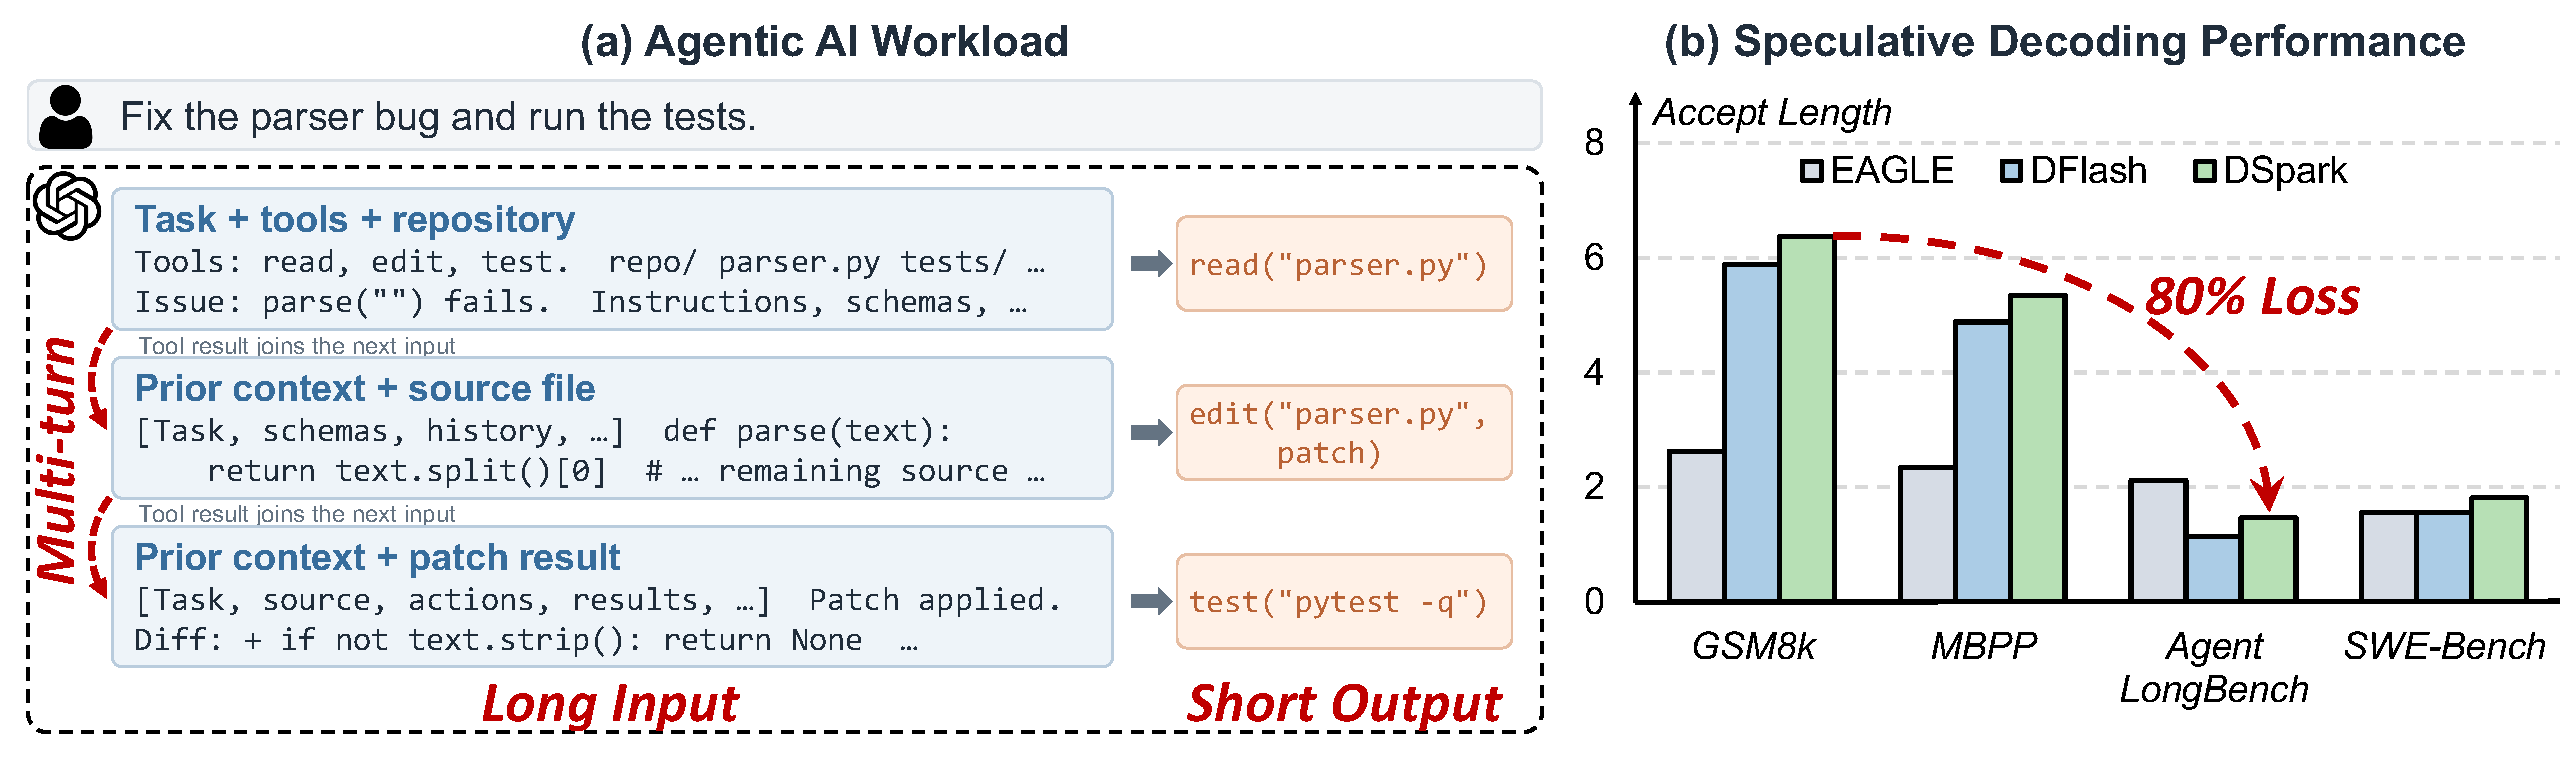
\includegraphics[width=0.98\textwidth]{fig/agent.pdf}
    \caption{(a) Agentic workloads characteristics. (b) Speculative decoding performance loss.}
    \vspace{-10pt}
    \label{fig:agent}
\end{figure}
% However, as agentic applications become increasingly mature, the computational workload characteristics handled by inference systems have fundamentally shifted. Unlike conventional requests in conversational AI, requests in agentic AI exhibit strong heterogeneity and runtime uncertainty in terms of context composition, sequence length, and execution paths due to the introduction of the harness~\cite{dsh}. This results in a unique workload profile: single-turn interactions typically feature long inputs but short outputs, while multi-turn interactions are characterized by high-frequency invocations and extended conversational depths. Under such workloads, we observe that existing state-of-the-art speculative decoding methods (\textit{e.g.}, EAGLE~\cite{li2024eagle}, DFlash~\cite{chen2026dflash}) encounter significant challenges in both algorithmic performance and system efficiency, even when deployed on mature LLM serving systems.

% \textbf{(1) From the perspective of algorithmic performance}, state-of-the-art speculative decoding methods can achieve substantial acceptance lengths on conventional workloads (\textit{e.g.}, DFlash achieves an acceptance length of nearly 6 on GSM8K~\cite{chen2026dflash}). However, under agentic workloads characterized by long inputs and short outputs, their performance degrades by over 80\%, with the acceptance length dropping to only $1\sim2$ tokens. This degradation substantially limits the acceleration potential of speculative decoding in agentic scenarios.

% \textbf{(2) From the perspective of system efficiency}, existing speculative decoding methods require the draft model to update its KV cache with the tokens accepted by the target model after verification to maintain consistency. Moreover, the draft model must synchronously maintain the complete historical KV cache alongside the target model to support prefix caching optimizations across similar requests. The high-frequency and multi-turn nature of agentic workloads makes these KV cache states particularly expensive to maintain and update. This overhead can account for $10\%\sim30\%$ in end-to-end inference latency.

% Our analysis reveals that these two problems share the same fundamental cause: the continuously growing historical context. On the one hand, a lightweight draft model with limited parameters fails to match the capability of the target model on the long-context understanding, leading to a degraded acceptance length. On the other hand, the inference system is persistently burdened with updating and maintaining the draft model's KV cache generated by this growing context, resulting in suboptimal system efficiency. To this end, we introduce \we, a speculative decoding framework tailored for agentic AI that jointly considers algorithmic performance and system efficiency from the outset.




% \textbf{(1) In the model design phase,} to ensure both algorithmic performance and system efficiency, \we adopts a lightweight semi-autoregressive architecture with a history-free design. Instead of maintaining the complete historical context cache, \we consists of a parallel backbone that performs prediction using only hidden states from the target model together with a local group of anchor tokens, and a lightweight serial head that explicitly models the sequential dependency among tokens within the speculative block. 

% \textbf{(2) In the model training phase,} to fully unlock the potential of this architecture, \we further introduces a tailored two-stage training strategy, the warm-up stage and stable stage, with different distillation targets and loss functions. During the warm-up stage, we first  train an isomorphic draft model equipped with historical context and use it as the distillation target for \we. \we is further trained to fit the output distribution using Kullback-Leibler (KL) divergence, with the goal of bringing the history-free model into a stable optimization region. Since the ultimate objective of the draft model is to align with the target model's output distribution, the stable stage shifts the distillation target directly to the target model. In this stage, \we is trained using a joint loss function of Cross-Entropy (CE) and Total Variation (TV) distance.

% We have trained the \we model for Qwen3-4B, Qwen3-8B, Qwen3.5-4B and evaluate them on NVIDIA H800 GPU. Extensive experiments demonstrate that \we achieves 2$\times \sim 6\times$ speedup on both general and agent-specific datasets, outperforming the state-of-the-art speculative decoding method, DSpark, by $20\% \sim 40\%$. Crucially, \we effectively enhances the acceptance length in agentic scenarios while entirely eliminating the system overhead associated with updating and maintaining the KV cache.






\section{Background}


% \begin{table}[!t]
% \centering
% \caption{The config of three typical drafters} \label{tab:latency}
% \begin{tabular}{@{}ccccc@{}}
% \toprule
% Architecture & EAGLE-3 (Autoregressive) & DFlash (Parallel) & DSpark (Semi-autoregressive) &  \\ \midrule
% Loss Function & KL divergence & Token-level CE & Token-level CE+TV &  \\ \midrule
% $\texttt{Time}_{M_D}(N)$ & $N \times L \times t$ & $L \times t$ & $L \times t + \gamma$ &  \\ \bottomrule
% \end{tabular}
% \end{table}

\subsection{Speculative Decoding}
% Speculative decoding accelerates LLM inference through a draft-and-verify pipeline. Given the current context, a lightweight draft model ($M_D$) generates $N$ candidate tokens ($\texttt{Time}_{M_D}(N)$), which are then verified in parallel ($\texttt{Time}_{M_T}(N)$) by the target model ($M_T$). The target model accepts a prefix of these candidates based on an acceptance criterion (\textit{e.g.}, rejection sampling) and typically recovers one additional token, totally generating $AL$ ($1 \sim N+1$) tokens by a single forward. Therefore, the practical speedup can be formulated  as follows~\cite{nvidiaspec}.
Speculative decoding accelerates LLM inference through a draft-and-verify pipeline shown in Figure~\ref{fig:background}(a). Given the current context, a lightweight draft model \(M_D\) generates \(N\) candidate tokens, which are subsequently verified in parallel by the target model \(M_T\). If \(\tau\) tokens are produced per verification round, the practical speedup~\cite{nvidiaspec} can be approximately expressed as

\begin{equation}
    \mathrm{Speedup} = \frac{\mathrm{Time}_{M_T}(1) \times \tau}{\mathrm{Time}_{M_T}(N)+\mathrm{Time}_{M_D}(N)}
\end{equation}

Therefore, speculative decoding performance mainly depends on two factors: acceptance length \(\tau\) and draft-model latency \(\mathrm{Time}_{M_D}(N)\).

Existing draft models mainly follow three architectural paradigms, summarized in Figure~\ref{fig:background}(b)(c)(d). Autoregressive drafters, represented by EAGLE~\cite{li2026eagle3}, explicitly preserve causal dependencies among speculative tokens but require sequential draft steps. Parallel drafters, such as DFlash~\cite{chen2026dflash}, predict all speculative positions in one forward pass, substantially reducing drafting latency but removing intra-block causal dependency. Semi-autoregressive drafters, including DSpark~\cite{cheng2026dspark} and Domino~\cite{huang2026domino}, combine a parallel backbone with a lightweight sequential module to balance drafting latency and prediction quality. Despite their different structures, these designs share one property: the draft model still explicitly depends on the historical context, whose length grows with decoding. In contrast, Figure~\ref{fig:background}(e) shows that \we removes this growing historical dependency by directly reusing contextual features produced by the target model and performs local prediction.

% Two important factors, $AL$ and $\texttt{Time}_{M_D}(N)$, depend on the capability and efficiency of the draft model, respectively. Therefore, various studies have explored many techniques to optimize these two factors. These studies can be broadly categorized into three model architecture paradigms, and the latency of these three architectures is formulated in Table~\ref{tab:latency}. The $L$ denotes the number of layers in the draft model, and the $t$ denotes the latency of executing a single transformer layer, and the $\gamma$ denotes the latency of executing the sequential module.

% \subsubsection{Autoregressive Architecture}
% Autoregressive drafters generate speculative tokens sequentially and explicitly model the causal dependency among draft tokens. EAGLE~\cite{li2024eagle,li2024eagle2,li2026eagle3} is the representative of this architecture, which leverages hidden states from the target model and employs a single transformer layer for autoregressive generation. Similar designs have also been introduced into industrial LLMs (\textit{e.g.}, DeepSeek-V4~\cite{xu2026deepseek} and GLM-5.2~\cite{zeng2026glm}) through native multi-token prediction (MTP) modules during post training. 
% The latency of these autoregressive draft models can be formulated as follows.

% \begin{equation}
%     \texttt{Time}_{M_D}(N) \approx N \times L \times t
% \end{equation}
% The $L$ denotes the number of layers in the draft model and the $t$ denotes the latency of executing a single transformer layer.


% \subsubsection{Parallel Architecture}
% To maximize execution efficiency, parallel drafters entirely eliminate the sequential generation dependency. The representative work, DFlash~\cite{chen2026dflash}, generates all $N$ candidate tokens simultaneously in a single forward pass on the current context. This design effectively reduce the latency and highly utilizes GPU parallelism. Therefore, this latency is formulated as follows.

% \begin{equation}
%     \texttt{Time}_{M_D}(N) \approx L \times t
% \end{equation}


% \subsubsection{Semi-autoregressive Architecture}
% Semi-autoregressive drafters aim to combine the advantages of the above two paradigms. DSpark~\cite{cheng2026dspark} and Domino~\cite{huang2026domino} employ a parallel backbone to efficiently model the speculative block like DFlash and introduce a lightweight sequential module to capture dependencies among draft tokens. In this way, the computationally expensive contextual modeling remains parallel, while only a lightweight component is executed sequentially. Such designs provide a better trade-off between acceptance quality and drafting latency, making semi-autoregressive drafting particularly attractive for practical serving systems. 

\begin{figure}[!t]
    \centering
    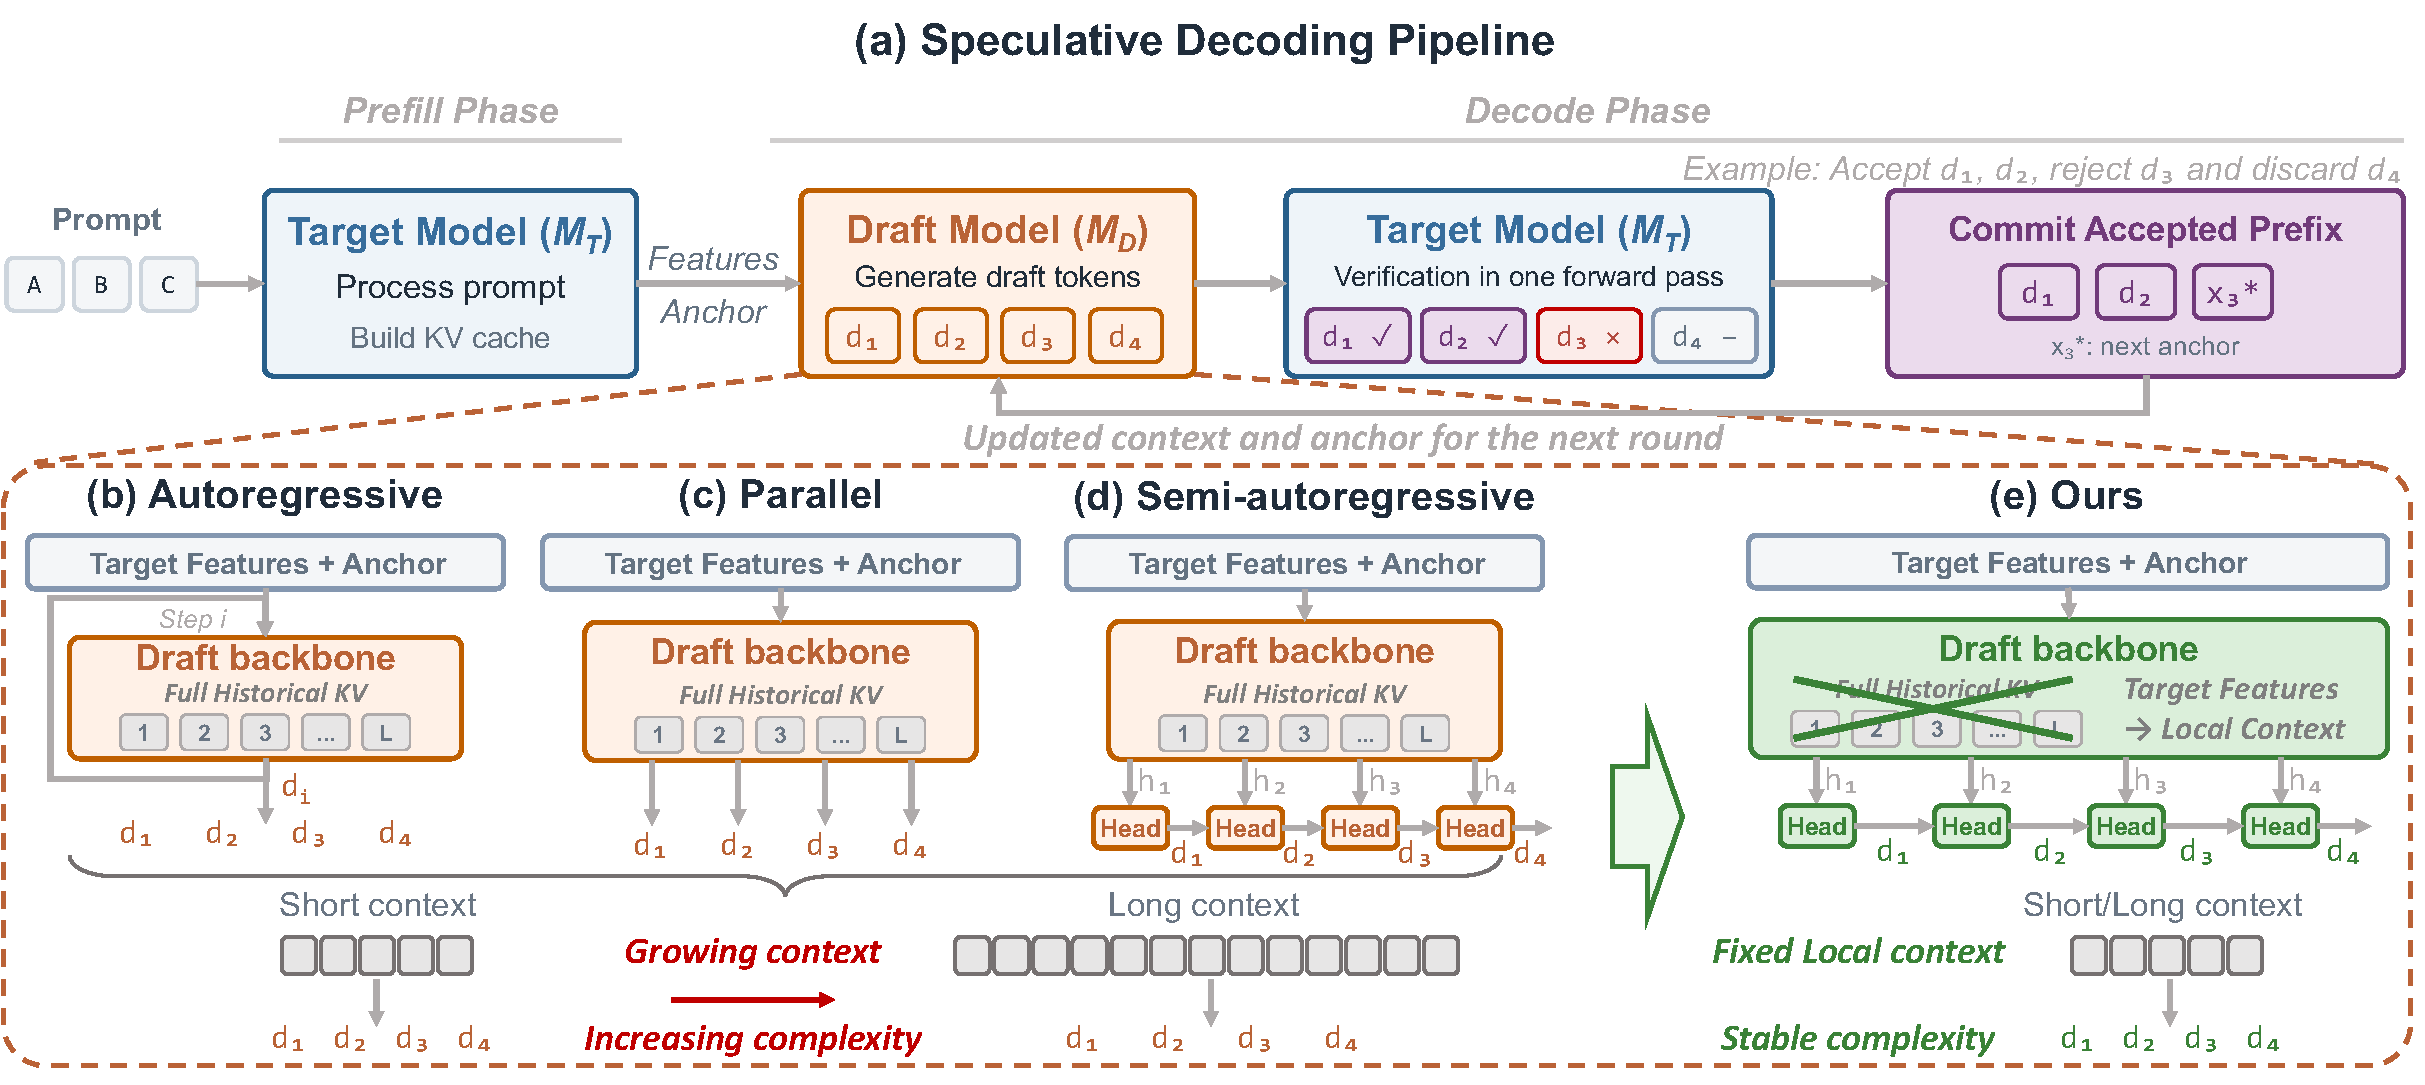
\includegraphics[width=0.98\textwidth]{fig/background2.pdf}
    % \vspace{-10pt}
    \caption{Speculative decoding pipeline and comparison of existing draft architectures with \we.}
    \label{fig:background}
    \vspace{-15pt}
\end{figure}



\subsection{Model Distillation}

Training a speculative draft model can be viewed as knowledge distillation from the target model. Different architectures adopt different supervision objectives. EAGLE performs distribution-level distillation using soft-target cross-entropy (CE), which is equivalent to minimizing forward Kullback-Leibler divergence up to a constant. DFlash primarily adopts token-level CE, while DSpark combines CE with total variation (TV) distance to improve distribution overlap between the draft and target models. Domino applies token-level supervision to both parallel and causally corrected predictions through a training curriculum. These differences are particularly relevant to \we because its history-free prediction structure differs substantially from the autoregressive target model, making direct distribution-level distillation non-trivial.

% The training of speculative draft models can be naturally viewed as knowledge distillation from the target model, while different drafting architectures adopt different supervision objectives. EAGLE~\cite{li2026eagle3} performs distribution-level distillation using soft-target cross-entropy ($\mathcal L_{\mathrm{cls}}=-\sum_v p_t(v)\log p_d(v)$), which is equivalent to minimizing the forward Kullback-Leibler divergence between the target and draft distributions up to the constant entropy of the target distribution. In contrast, DFlash~\cite{chen2026dflash} primarily trains its parallel draft model using position-weighted token-level cross-entropy ($\mathcal L_{\mathrm{CE}}=-\sum_k w_k \log q_k(x_k)$), while DSpark~\cite{cheng2026dspark} further combines cross-entropy with total variation (TV) distance ($\mathcal L_{\mathrm{TV}}=\sum_k w_k\|p_k^d-p_k^t\|_1$) to directly improve the distribution overlap that determines speculative acceptance. Domino~\cite{huang2026domino} jointly applies token-level cross-entropy to the parallel backbone and the causally corrected predictions with a training curriculum that gradually shifts optimization toward the latter. 

% Although forward KL is widely adopted in conventional knowledge distillation, directly applying distribution-level distillation becomes less natural for parallel and semi-autoregressive drafters because their prediction structures and conditioning information are different from those of the autoregressive target model. The difficulty is therefore not that heterogeneous architectures mathematically prevent KL-based distillation, but that the target and draft distributions are produced under different conditioning structures, making direct distribution alignment less effective. Consequently, these methods typically rely more heavily on token-level supervision and introduce architecture- or acceptance-aware objectives to train their draft models.






\section{Motivation} \label{sec:motivation}

\subsection{Two Important Observations}

Agentic workloads expose two limitations of existing speculative decoding methods: degraded acceptance length and increasing historical-state maintenance overhead.

% As illustrated in Figure~\ref{fig:agent}(a), agents introduce workload characteristics substantially different from conventional conversational inference. With the orchestration of agent harness framework, a single task typically consists of frequent multi-turn LLM interactions with heterogeneous context compositions and execution trajectories. Each turn is often characterized by a long input and a short output, while the accumulated context continuously grows across turns. We find that these workload characteristics expose two major limitations of existing speculative decoding methods.

\textbf{Degraded Acceptance Length.} As illustrated in Figure~\ref{fig:agent}(b), existing speculative decoding methods achieve high acceptance lengths on general workloads such as GSM8K and MBPP, but degrade substantially on agentic workloads such as SWE-Bench and AgentLongBench. As the context grows, lightweight draft models increasingly struggle to capture the information required to match the target model's predictions, causing acceptance lengths to drop to only \(1\sim2\) tokens in some workloads.

% State-of-the-art speculative decoding (\textit{e.g.}, EAGLE~\cite{li2024eagle}, DFlash~\cite{chen2026dflash}, DSpark~\cite{cheng2026dspark}) methods achieve high acceptance lengths on conventional general benchmarks (\textit{e.g.,} GSM8K and MBPP), but their performance degrades significantly under agentic workloads (\textit{e.g.}, SWE-Bench and Agent LongBench). We point out that, as the context grows, lightweight draft models increasingly struggle to capture the information required for accurate prediction, causing their output distributions to deviate from the target model. Figure~\ref{fig:agent}(b) shows that methods that achieve high acceptance lengths on general workloads drop to only $1\sim2$ accepted tokens on agentic workloads with over 80\% performance loss.

\textbf{KV Cache Maintenance.} Existing speculative drafters must maintain historical KV states for subsequent generation. After each target-model verification, accepted tokens are committed to the draft model to update its KV cache, while prefix caching further requires historical draft states to be preserved across agent turns. Under frequent multi-turn workloads with continuously growing contexts, these operations become increasingly expensive. Using SGLang to evaluate the multi-token prediction module in DeepSeek-V4, we observe that the KV cache  updating and maintenance can account for \(10\%\sim20\%\) of end-to-end inference latency.

% As illustrated in Figure~\ref{fig:background}(a), after the verification in target-model, accepted tokens must be committed to the draft model to update its KV cache to maintain the consistency for subsequent draft generation. Under agentic workloads, frequent short generations and continuously growing contexts make such updates particularly expensive. Moreover, supporting prefix caching across multiple agent turns requires the draft model to retain and manage its own historical KV cache regardless of full attention and sliding window attention. We use SGLang~\cite{zheng2024sglang} to evaluate the overhead of the multi-token prediction module in DeepSeek-V4, and find that the updating and maintenance operations can account for $10\%\sim30\%$ of end-to-end inference latency, significantly reducing the system-level benefit of speculative decoding.


\subsection{Analysis and Findings}

% Although the above limitations manifest differently at the model and system levels, our analysis reveals a common root cause: the \emph{growing historical context}. From the model perspective, existing draft models attempt to independently encode an increasingly long history with only a small fraction of the target model's parameters. The resulting gap in long-context modeling capability leads to progressively less accurate draft predictions and lower acceptance lengths. From the system perspective, preserving the same history requires maintaining an ever-growing KV cache for the draft model, which must be repeatedly updated and managed throughout multi-round agent execution.

% These observations expose a fundamental inefficiency in existing speculative decoding: the lightweight draft model is required to both \emph{understand} and \emph{maintain} the complete historical context, even though the target model has already processed the same context and encoded it into its internal representations. This motivates a different design principle for Agentic workloads: rather than independently reconstructing historical information within the draft model, the drafter should directly exploit the contextual representations produced by the target model and operate without maintaining its own historical context cache.

% Based on this insight, we design \we as a \emph{history-free} speculative decoding framework that removes the draft model's dependence on historical KV cache while preserving the contextual information required for accurate speculation.

Although the above problems appear at different levels, they share a common cause: the draft model is required to independently process and maintain the growing historical context shown in Figure~\ref{fig:background}. From the model perspective, a lightweight drafter has only a fraction of the target model's capacity, making it increasingly difficult to reproduce the target model's long-context representation as history grows. From the system perspective, preserving the same history requires maintaining and repeatedly updating an increasingly large draft KV cache.

The key inefficiency is therefore that the draft model repeatedly reconstructs historical information that has already been processed by the target model. We instead argue that the drafter should directly reuse the target model's contextual representations and dedicate its limited capacity to modeling the information required for local speculative prediction. 
% This observation motivates \we, which removes the draft model's dependence on historical KV cache by directly reusing target hidden states for contextual information and performing only local speculative prediction shown in Figure~\ref{fig:background}(e).




\section{\we Framework}

Motivated by the observations in Section~\ref{sec:motivation}, we design \we to decouple historical-context modeling from speculative generation. As illustrated in Figure~\ref{fig:background}(e), instead of requiring a lightweight draft model to repeatedly process and maintain an ever-growing history, \we delegates global-context modeling to the target model and performs drafting only over compact target hidden states. This design transforms speculative drafting \textbf{from an increasingly complex growing-history modeling problem into a local prediction problem} whose structure and positional range remain independent of the accumulated sequence length. \we realizes this principle through a history-free semi-autoregressive architecture and a two-stage training strategy.

% v2
% Motivated by the findings in Section~\ref{sec:motivation}, \we decouples historical-context modeling from speculative generation. The target model remains responsible for processing the complete context, while the draft model operates only on compact target representations and a sliding anchor group. \we consists of two key components: a history-free semi-autoregressive architecture for efficient speculative generation and a two-stage training strategy for effectively training the history-free drafter.


% v1
% The key design principle of \we is to avoid repeatedly encoding and maintaining the complete historical context within the draft model. Instead, \we directly reuses contextual hidden states produced by the target model and performs speculation only over a sliding anchor group. To achieve both high drafting quality and low execution overhead, \we is built upon a history-free semi-autoregressive architecture in Section~\ref{sec:DLite:arch} and is further trained through the specific two-stage strategy in Section~\ref{sec:DLite:train}. 
% In the following, we first introduce the History-Free Semi-Autoregressive Architecture, followed by the Two-Stage Training Strategy.


\subsection{History-free semi-autoregressive Architecture} \label{sec:DLite:arch}

Figure~\ref{fig:overview} illustrates the inference dataflow of \we. The target model first processes the input context and maintains its original KV cache. For each speculative round, \we takes contextual hidden states from the target model, the current anchor token, and \(K\) draft placeholders as input. A history-free parallel backbone produces hidden representations for all speculative positions simultaneously, after which a lightweight sequential head restores the causal dependency among tokens within the speculative block. The resulting candidate tokens are finally verified by the target model following the standard speculative decoding procedure. It is worth noting that \we maintains no historical draft KV cache throughout this process. Each speculative round is independently reconstructed from the latest target representations and the current anchor token, allowing the drafter to perform prediction locally without explicitly processing the accumulated history.


% v2
% Figure~\ref{fig:overview} illustrates the inference workflow of \we. The target model first processes the input context and maintains its original KV cache. For each speculative round, \we takes target hidden states, a small sliding anchor group, and \(K\) draft placeholders as input. A history-free parallel backbone produces hidden representations for all speculative positions simultaneously, after which a lightweight sequential head restores the causal dependency among tokens within the speculative block. The resulting draft tokens are finally verified by the target model in the standard speculative-decoding pipeline. It is worth noting that, unlike conventional drafters, \we maintains no historical draft KV cache throughout this process.

% v1
% Figure~\ref{fig:overview} illustrates the overall inference workflow and architecture of \we. \we adopts a history-free semi-autoregressive design that directly reuses contextual representations produced by the target model, instead of maintaining an independent historical KV cache for the draft model. The architecture consists of two components: \textbf{a history-free parallel backbone} and \textbf{a lightweight sequential head}.

% Given an input prompt, the target model first performs standard prefill operation and maintains its original KV cache. The parallel backbone then takes hidden states extracted from the target model, the sliding anchor group, and several draft placeholders as input, and produces hidden states for multiple speculative positions in parallel. A lightweight sequential head further introduces causal dependencies among the speculative tokens before they are verified by the target model. During this process, \we will \textbf{not} store any historical KV cache.

\begin{figure}[!t]
    \centering
    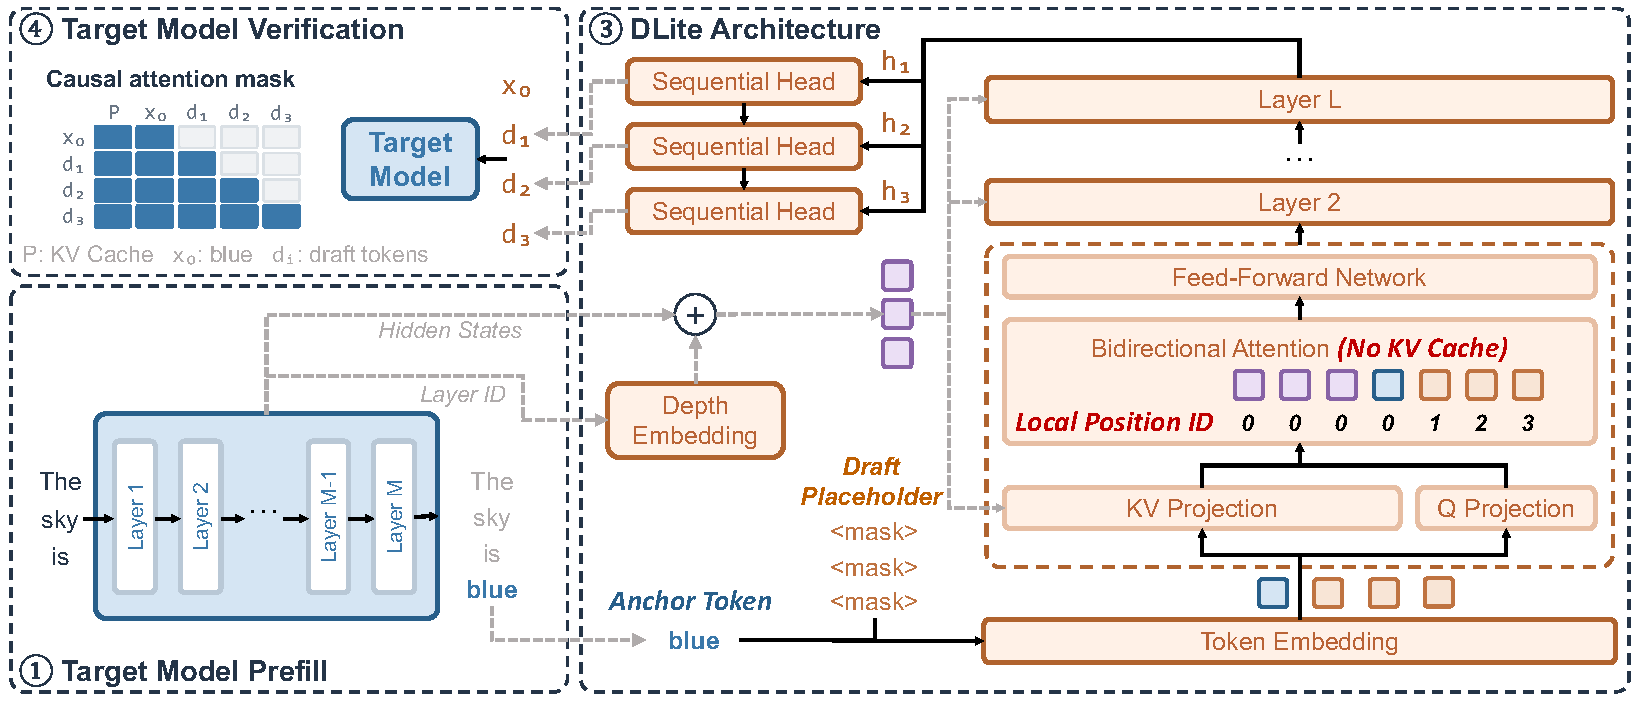
\includegraphics[width=0.98\textwidth]{fig/overview2.pdf}
    \vspace{-5pt}
    \caption{The inference dataflow of \we.}
    \label{fig:overview}
    \vspace{-10pt}
\end{figure} 

\subsubsection{History-free Parallel Backbone}

The key idea of the history-free parallel backbone is to \textbf{transform speculative drafting from growing-history modeling into local prediction}. To this end, the backbone combines compact target hidden states with explicit local token information and performs local prediction.


% v2
% The parallel backbone is designed to extract sufficient contextual information for speculation without independently reconstructing the full historical context. It combines three sources of information: target hidden states, a sliding anchor group, and local positional information.


\textbf{Target hidden states.} \we directly reuses hidden states produced by the target model as compact contextual features. Since target hidden states and ordinary token embeddings correspond to different input sources, we introduce a learnable depth embedding to distinguish them. When hidden states from multiple target layers are used, the same embedding also identifies their source layers. For a target hidden state \(h_t^{(l)}\) extracted from layer \(l\), we construct
\begin{equation}
    z_t^{(l)} = h_t^{(l)} + e_{\mathrm{depth}}^{(l)}
\end{equation}
where \(e_{\mathrm{depth}}^{(l)}\) is a learnable source-specific embedding.

% \textbf{Sliding anchor group.} Target hidden states provide a compact representation of the historical context, but may lose fine-grained information about the most recent tokens. \we therefore retains a small sliding anchor group around the current decoding position to provide explicit local token information. As decoding proceeds, the anchor group moves forward with the accepted prefix. Its size remains fixed, allowing the backbone to preserve fine-grained short-range context without introducing a growing historical state.


\textbf{Local prediction.} Conventional drafters operate over an ever-growing history, such that both the explicit context and global positions increase as decoding proceeds. \we instead delegates long-context modeling to the target model and performs draft prediction only around the current decoding position. The backbone takes the current anchor token and \(K\) speculative positions, while using local rather than globally accumulated positions. Historical information is retained through the target hidden states, allowing the drafter to focus on local prediction without explicitly reconstructing the history. \we therefore transforms growing-history modeling into a local prediction problem. 

% \textbf{Fixed-size local prediction.} Conventional speculative drafters operate on an ever-growing historical sequence. At decoding position \(t\), the drafter must predict future tokens conditioned on $x_{<t}$ whose length and associated global positions continuously increase as decoding proceeds. For a lightweight draft model, the structure of the prediction problem therefore becomes increasingly demanding as the historical context grows. 

% \we removes this dependence by delegating long-context hidden states to the target model. Given the compressed target hidden states and a fixed-size anchor group of size \(A\), the draft backbone only operates over a local prediction window containing \(A\) anchor tokens and \(K\) speculative positions. Accordingly, \we assigns positions relative to the current local window rather than using globally accumulated positions. The positional range is always

% \begin{equation}
%  \{0,1,\ldots,A+K-1\}
% \end{equation}

% regardless of whether the original sequence contains thousands or hundreds of thousands of tokens.

% Therefore, as the sequence grows, the structural complexity of the draft-side prediction problem remains bounded: both the explicit token context and positional range seen by the backbone remain fixed. \we thus converts an increasingly long-context prediction problem into \textbf{a fixed-size local prediction problem that is independent of the accumulated sequence length}.

% Each speculative round is consequently reconstructed from the current target hidden states, sliding anchors, and draft placeholders without caching historical backbone states. Formally, given the target features \(\mathcal{Z}_t\), anchor group \(A_t\), and \(K\) draft placeholders \(M_{1:K}\), the parallel backbone produces

% \begin{equation}
% (h_1,h_2,\ldots,h_K) = F_{\theta} \left( \mathcal{Z}_t, A_t, M_{1:K} \right)
% \end{equation}

% where \(h_T\) denotes the hidden states corresponding to the \(T\)-th speculative position. All \(K\) representations are computed in parallel using bidirectional attention within the local window.


% v2
% \textbf{History-free computation and local positions.} Unlike conventional speculative drafters, \we does not cache any historical backbone states. Each speculative round is reconstructed from the current target hidden states, sliding anchors, and draft placeholders. Therefore, the draft-side state does not grow with the accumulated sequence history.

% To match this history-free computation, \we uses local position embeddings within the current speculative window rather than globally accumulated sequence positions. Positions are defined only relative to the local anchor-and-draft window, so each speculative round is formulated as a fixed-size local prediction problem independent of the absolute sequence position.

% Given the target features \(\mathcal{Z}_t\), anchor group \(A_t\), and \(K\) draft placeholders \(M_{1:K}\), the parallel backbone produces
% \begin{equation}
%     (h_1,h_2,\ldots,h_K) = F_{\theta} \left( \mathcal{Z}_t, A_t, M_{1:K} \right) 
% \end{equation}
% where \(h_T\) denotes the backbone representation for the \(T\)-th speculative position.


% The history-free parallel backbone is the core component that enables \we to perform efficient speculative drafting without maintaining a historical KV cache. Its design is built on four key ideas: depth-aware target features, a sliding anchor group, history-free computation without KV cache, and local position encoding.

% First, \we directly reuses hidden states from the target model as compact contextual inputs. Since hidden representations from different target layers capture complementary semantic information, \we introduces a learnable depth embedding to encode the source-layer identity of each extracted hidden state. Specifically, for the hidden state \(h_t^{(l)}\) taken from target layer \(l\), we construct a depth-aware feature as
% \begin{equation}
%     z_t^{(l)} = h_t^{(l)} + e_{\mathrm{depth}}^{(l)}
% \end{equation}

% where \(e_{\mathrm{depth}}^{(l)}\) is a learnable source-specific embedding. This embedding allows the backbone to distinguish token embeddings from target hidden states and, when multiple target layers are used, to distinguish hidden states originating from different depths, rather than treating all inputs as homogeneous representations.

% Second, \we introduces a sliding anchor group composed of a small number of recent tokens near the current decoding position. While the target hidden states provide a compressed representation of the full historical context, the anchor group preserves fine-grained local token information that is especially useful for short-range continuation. As decoding proceeds, this anchor group slides forward with the accepted prefix, ensuring that the backbone always conditions on the most relevant local context while keeping the input length fixed.

% Third, unlike conventional speculative drafters, the \we backbone performs history-free computation without maintaining any draft KV cache. Existing methods typically preserve historical draft states and incrementally update them after each verification step, which incurs additional synchronization and maintenance overhead. In contrast, \we reconstructs each speculative round from scratch using only the current target features, the sliding anchor group, and several draft placeholders. As a result, the computational and memory cost of the backbone is independent of the accumulated decoding history.

% Finally, to match this history-free design, \we adopts local position embeddings within the current speculative window, rather than absolute or globally accumulated positions over the full sequence. The anchor tokens and speculative placeholders are assigned positions only relative to the current local window. This local position scheme allows the backbone to focus on short-range structural relationships among the anchor group and speculative positions, while avoiding any dependence on the absolute sequence length. It also naturally aligns with the no-KV-cache design, since each speculative round is computed as an independent local prediction problem.

% Based on these designs, the backbone takes as input the depth-aware target features, the sliding anchor group, and the draft placeholders, and applies bidirectional attention to produce hidden representations for all speculative positions in parallel:

% $$ h_1, h_2, \ldots, h_K . $$

% These representations summarize both the global contextual information extracted from the target model and the local structural information encoded within the speculative window, and are then passed to the lightweight sequential head for causal refinement.


\subsubsection{Lightweight Sequential Head}


While the parallel backbone efficiently produces representations for multiple speculative positions, parallel computation removes the autoregressive dependency among tokens within the speculative block. \we therefore introduces a lightweight sequential head that \textbf{restores only the missing intra-block dependency}, rather than performing another full contextual modeling process.


Let \(t\) denote the starting position of a speculative block and \(T\) the intra-block offset. The target model predicts \(x_{t+T}\) autoregressively according to
\begin{equation}
p_T \left( x_{t+T}\mid x_{<t+T} \right) = p_T \left( x_{t+T} \mid x_{<t}, x_{t:t+T-1} \right) 
\end{equation}
The parallel backbone, however, produces \(h_T\) before the tokens at earlier speculative positions are sampled. Since the preceding context \(x_{<t}\) has already been processed by the target model and conveyed through its contextual representations into \(h_T\), the information missing from parallel drafting is precisely the intra-block prefix $ x_{t:t+T-1}$. This decomposition suggests that the sequential module does not need to reconstruct the complete historical context. It only needs to encode tokens generated earlier within the current speculative block.

To recover this missing dependency efficiently, we employ a low-rank RNN-style sequential head. It recursively compresses previously generated draft tokens into a recurrent state
\begin{equation}
s_T = g_{\phi} \left( s_{T-1}, E(x_{t+T-1}) \right)
\end{equation}
where \(E(\cdot)\) denotes the token embedding. The prediction at speculative position \(T\) is modeled as
\begin{equation}
q_{\theta,\phi} \left( x_{t+T}\mid h_T,s_T \right) \approx p_T \left( x_{t+T} \mid x_{<t}, x_{t:t+T-1} \right)
\end{equation}
Here, \(h_T\) supplies the contextual information already encoded by the target model, while \(s_T\) summarizes the missing intra-block prefix. Together, they recover the information required for autoregressive prediction without reconstructing the full history inside the draft model. This preserves most contextual computation in the parallel backbone while restricting sequential execution to a lightweight low-rank module.

Furthermore, unlike existing semi-autoregressive methods that first project every backbone representation into full-vocabulary logits and subsequently refine these predictions with an additional sequential module, \we performs sequential modeling directly in the hidden space. The vocabulary projection is applied only after the intra-block dependency has been incorporated.

For hidden dimension \(D\) and vocabulary size \(V\), this avoids repeatedly applying an intermediate \(D\times V\) projection to every speculative representation before sequential refinement. Such computation becomes particularly expensive under high-concurrency serving, where a large number of speculative hidden states are processed simultaneously.



% v2
% Parallel drafting reduces draft latency by predicting multiple speculative positions simultaneously. However, this parallelism removes the auto-regressive dependency among speculative positions, causing prediction quality to degrade at deeper draft positions. As observed by DSpark, explicitly restoring \textbf{intra-block sequential dependency} is important for maintaining high acceptance rates. Following this insight, we introduce a sequential decoding stage on top of the parallel backbone. Unlike existing methods that first project each backbone hidden state into full-vocabulary logits and then employ an additional sequential head to refine these predictions, we find that the expensive vocabulary projection is unnecessary for draft prediction.

% Let $t$ denote the starting position of a speculative block and $T$ denote the intra-block offset. The target model predicts \(x_{t+T}\) auto regressively according to $p(x_{t+T} \mid x_{<t}, x_{t:t+T-1})$. In contrast, the parallel backbone produces a hidden representation $h_T$ without observing the tokens sampled at earlier positions within the same block. In \we, the preceding context \(x_{<t}\) is compactly conveyed through the target representation \(H_t\) and encoded into \(h_T\). To align with the target model’s auto-regressive formulation, the missing information in parallel drafting is precisely the intra-block prefix token \(x_{t:t+T-1}\).

% To efficiently recover this missing dependency, we employ a low-rank RNN-style head that recursively compresses previously generated draft tokens within the draft block into a recurrent state: 
% $s_T = RNN(s_{T-1}, x_{t+T-1})$. 
% The prediction at position \(T\) is then directly modeled as
% $ q_\theta(x_{t+T}\mid h_T,s_T) \approx p(x_{t+T}\mid x_{<t},x_{t:t+T-1}).$ Here, \(s_T\) summarizes the intra-block prefix. Together, they recover the information required for autoregressive prediction.

% This formulation also avoids the expensive intermediate vocabulary projection used by existing sequential-refinement methods. Instead of first projecting each \(D\)-dimensional backbone hidden state into \(V\)-dimensional logits and then refining these logits with an additional sequential module, \we restores the missing sequential dependency directly in the low-rank hidden space. This is particularly important for high-concurrency serving, where repeatedly applying a \(D\times V\) vocabulary projection to a large batch of speculative hidden states can become a significant drafting bottleneck. 

% In Exp Section, Our method can reduce the draft latency by 70\%, leading to 10\% - 20\% throughput improvement under multi-request scenario.



\begin{figure}[!t]
    \centering
    \vspace{-12pt}
    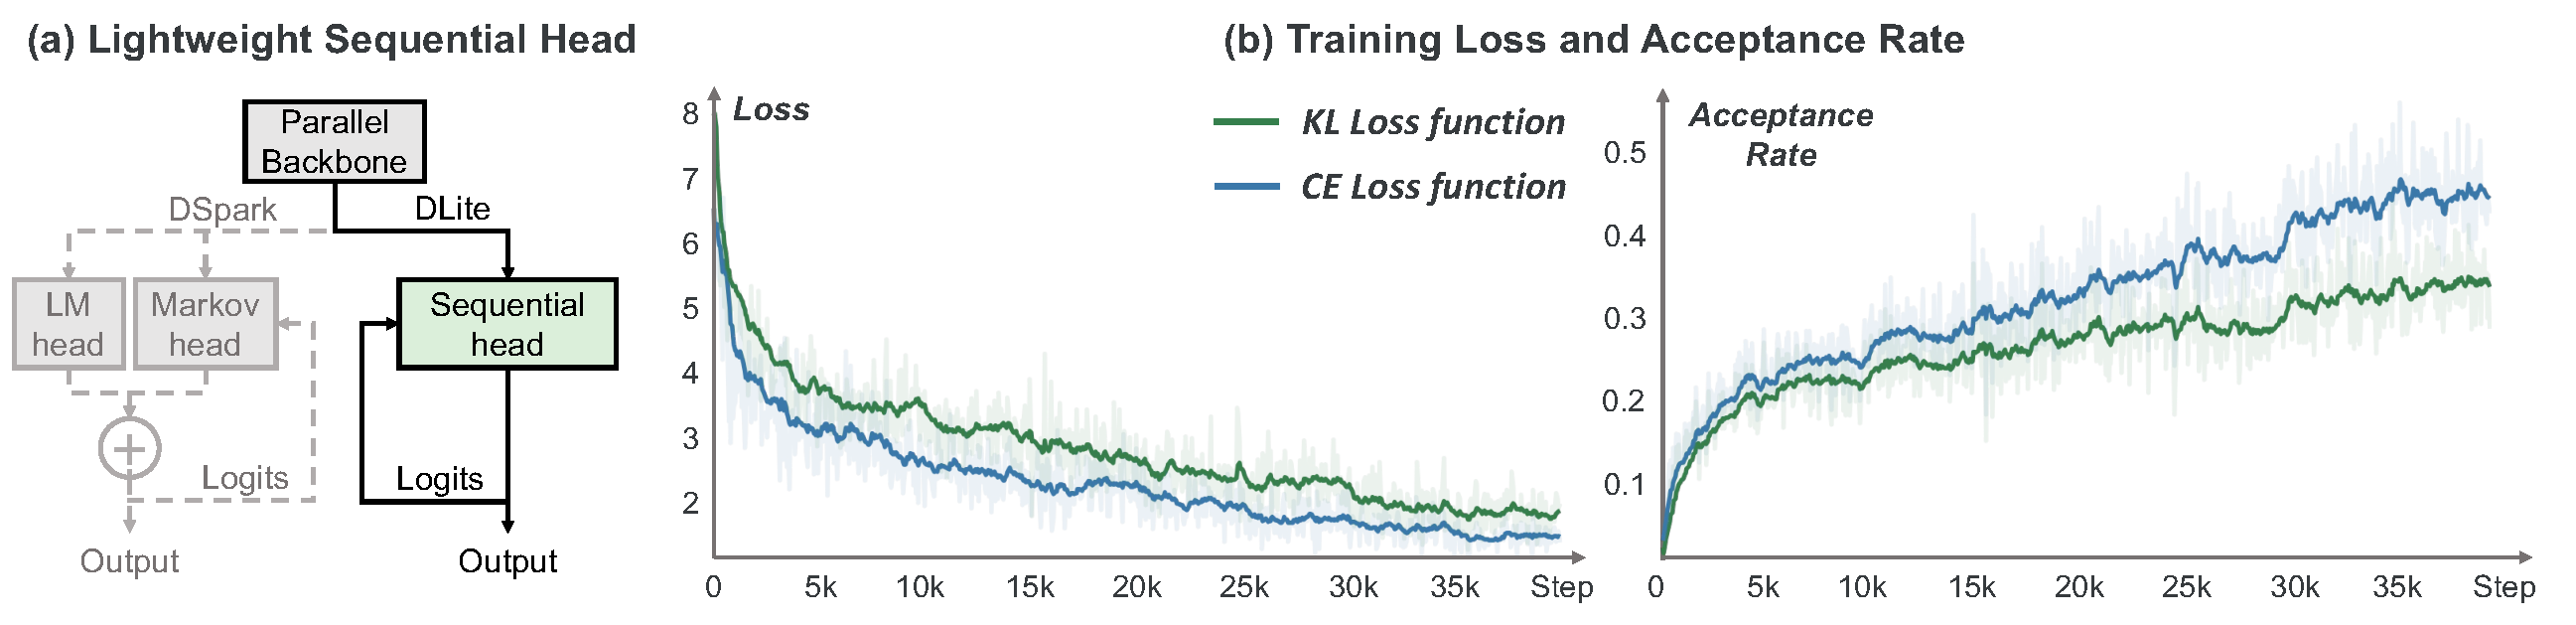
\includegraphics[width=\linewidth]{fig/training.pdf}
    \caption{(a) The design architecture of the lightweight sequential head. (b) The training loss and acceptance rate curves of direct target-model distillation using KL and CE loss function.}
    \label{fig:train}
    \vspace{-15pt}
\end{figure}


\subsection{Two-stage Training Strategy} \label{sec:DLite:train}
The objective of a speculative draft model is to approximate the predictive distribution of the target model, since a larger distribution overlap generally leads to a higher speculative acceptance probability. Distribution-level objectives such as KL divergence are therefore natural choices for distillation. However, Figure~\ref{fig:train}(b) shows that directly applying KL distillation from the target model to the parallel backbone in \we performs poorly. The two models make predictions under substantially different conditions: the target model performs autoregressive prediction over the complete historical context, whereas the backbone performs parallel prediction using compressed target hidden states,
% Consequently, their output distributions are induced by heterogeneous prediction structures and conditioning information, 
making direct distribution alignment difficult. To bridge this structural gap, we introduce a two-stage training strategy. The warm-up stage first trains \we against an isomorphic history-aware teacher, providing a structurally matched intermediate distillation target. The stable stage subsequently removes this teacher and directly aligns \we with the original target model. Let \(K\) denote the speculative block length and \(V\) the vocabulary size. At speculative position \(i\), we denote the predictive distributions of the target model, history-aware teacher, and \we as $p_i^T, p_i^H, q_i$ respectively, and denote the ground-truth token as \(y_i\).


% v2
% The ultimate objective of a speculative draft model is to approximate the predictive distribution of the target model, since a larger overlap between the two distributions generally leads to a higher acceptance probability. Compared with hard-label cross-entropy, which only supervises the probability assigned to the observed token, KL divergence provides dense supervision over the entire target distribution and is therefore a natural objective for distribution-level distillation. However, Figure~\ref{fig:train}(b) shows that directly applying KL distillation between \we and the target model performs poorly in our experiments. We attribute this difficulty to the substantial mismatch between their prediction structures and conditioning information: the target model performs autoregressive prediction over the complete historical context, whereas \we performs history-free block prediction using compressed target features and local tokens. Consequently, the two distributions are induced under heterogeneous prediction conditions, making direct distribution alignment difficult.

% To effectively exploit distribution-level supervision while addressing this structural mismatch, we introduce a two-stage training strategy. The first stage constructs a history-aware model that is architecturally aligned with \we and uses it as an intermediate teacher for KL distillation. The second stage removes this intermediate teacher and directly aligns \we with the original target model using objectives that are better aligned with speculative acceptance.

% Let \(K\) denote the speculative block length and \(\mathcal{V}\) the vocabulary. For the \(i\)-th speculative position, we denote the output distributions of the target model, the history-aware teacher, and \we as \(p_i^{T}\), \(p_i^{H}\), and \(q_i\), respectively, and denote the supervision token as \(y_i\).



% \subsubsection{Warm-up Stage}


\textbf{Warm-up Stage.} In the warm-up stage, we first train an isomorphic history-aware teacher by standard token-level cross-entropy (\(-\sum_i w_i \ \mathrm{log}\ {p_i^H(y_i)}\)). The teacher shares the same backbone and prediction structure as \we, but retains access to historical KV cache. 
% Since this teacher does not need to learn history-free prediction from the beginning, it can be effectively optimized with .
% \[
% \mathcal{L}_{\mathrm{teacher}}
% =
% \mathcal{L}_{\mathrm{CE}}
% =
% -\frac{1}{K}
% \sum_{i=1}^{K}
% \log p_i^{H}(y_i).
% \]
Once the history-aware teacher is sufficiently trained, we use it as an intermediate distillation target for \we using forward KL divergence: 
\begin{equation}
\mathcal{L}_{\mathrm{warmup}}
=
\sum_{i=1}^{K}
w_i D_{\mathrm{KL}}
\left(
p_i^{H}\,\|\,q_i
\right)
=
\sum_{i=1}^{K}
w_i
\sum_{v\in\mathcal V}
p_i^{H}(v)
\log
\frac{p_i^{H}(v)}
{q_i(v)}
\end{equation}
where \(w_i = \exp(\frac{-(i-1)}{\gamma})\) emphasizes the contribution of earlier positions. Because the teacher and \we share the same architecture and prediction interface, their output distributions are naturally aligned despite the difference in historical information available to them.

The history-aware teacher therefore serves as an optimization bridge between the autoregressive target model and the history-free drafter. Instead of forcing \we to directly match a target distribution, the warm-up stage first exposes it to a structurally matched predictive distribution, providing a more stable starting point for subsequent target-model alignment.


%v2
% In the warmup stage, we first train an isomorphic history-aware teacher that shares the same backbone and prediction structure as \we, but retains access to historical KV cache. Since this teacher does not need to learn history-free prediction from the beginning, it can be effectively optimized with standard token-level cross-entropy:
% \[
% \mathcal{L}_{\mathrm{teacher}}
% =
% \mathcal{L}_{\mathrm{CE}}
% =
% -\frac{1}{K}
% \sum_{i=1}^{K}
% \log p_i^{H}(y_i).
% \]Once the history-aware teacher is sufficiently trained, we use it as an intermediate distillation target for \we. Because the teacher and \we share the same architecture and prediction interface, their output distributions are naturally aligned despite the difference in historical information available to them. We therefore optimize \we using forward KL divergence:
% \[
% \mathcal{L}_{\mathrm{warmup}}
% =
% \frac{1}{K}
% \sum_{i=1}^{K}
% D_{\mathrm{KL}}
% \left(
% p_i^{H}\,\|\,q_i
% \right)
% =
% \frac{1}{K}
% \sum_{v\in\mathcal V}
% p_i^{H}(v)
% \log
% \frac{p_i^{H}(v)}
% {q_i(v)}.
% \]Instead of forcing the history-free model to directly match the substantially different target model from the beginning, this stage uses the history-aware isomorphic teacher as an optimization bridge, guiding \we toward a stable parameter region while progressively transferring the predictive capability obtained from historical context into the history-free architecture.


% \subsubsection{Stable Stage}


\textbf{Stable Stage.} Although the intermediate teacher facilitates optimization, the ultimate objective of \we is to match the predictive distribution of the target model. We therefore discard the history-aware teacher 
in the stable stage and directly optimize \we against the target model using
\begin{equation}
\mathcal L_{\mathrm{stable}} = \lambda_{\mathrm{CE}}\mathcal L_{\mathrm{CE}} + \lambda_{\mathrm{TV}}\mathcal L_{\mathrm{TV}}
\end{equation}
where \(\mathcal L_{\mathrm{CE}}\) denotes token-level cross-entropy and
\(\mathcal L_{\mathrm{TV}}=\sum_i w_i \|p_i^T-q_i\|_1\) measures target–draft distribution discrepancy. 

% Following the objective of maximizing distribution overlap relevant to speculative acceptance, we combine token-level cross-entropy with total variation (TV) distance. The cross-entropy loss is
% \begin{equation}
% \mathcal{L}_{\mathrm{CE}} = -\frac{1}{K} \sum_{i=1}^{K} \log q_i(y_i)
% \end{equation}

% and the TV-based distribution alignment objective is
% \begin{equation}
% \mathcal{L}_{\mathrm{TV}} = \frac{1}{K} \sum_{i=1}^{K} \left\| p_i^T-q_i \right\|_1
% \end{equation}
% The final training objective is
% \begin{equation}
% \mathcal{L}_{\mathrm{stable}} = \lambda_{\mathrm{CE}} \mathcal{L}_{\mathrm{CE}} + \lambda_{\mathrm{TV}} \mathcal{L}_{\mathrm{TV}}
% \end{equation}

% where \(\lambda_{\mathrm{CE}}\) and \(\lambda_{\mathrm{TV}}\) control the relative contributions of token-level supervision and distribution alignment.

% In this stage, DLite is no longer constrained by the intermediate teacher and is directly optimized toward the target-model distribution that determines speculative acceptance. Together, the two stages progressively transition the history-free drafter from a structurally aligned intermediate teacher to the original target model.


% v2
% Although the history-aware teacher provides an effective intermediate target, the ultimate objective of \we is to match the original target model rather than the auxiliary teacher. We therefore discard the history-aware teacher in the stable stage and directly optimize \we against the target model.
% Specifically, we combine token-level cross-entropy with total variation (TV) distance like DSpark in Table~\ref{tab:latency}. The final objective of the stable stage is therefore
% \[
% \mathcal{L}_{\mathrm{stable}}
% =
% \lambda_{\mathrm{CE}}
% \mathcal{L}_{\mathrm{CE}}
% +
% \lambda_{\mathrm{TV}}
% \mathcal{L}_{\mathrm{TV}},
% \]where \(\lambda_{\mathrm{CE}}\) and \(\lambda_{\mathrm{TV}}\) control the relative contributions of token-level supervision and distribution alignment. 




\section{Experiments}
\begin{table}[!t]
\centering
\caption{Acceptance length $\tau$ evaluation on general-purpose workloads.}
\label{tab:acceptance_length}
\small
\setlength{\tabcolsep}{4.2pt} % <--- 增加一列后内容变宽，适当调小列间距
\renewcommand{\arraystretch}{1.1}
\begin{tabular}{llccccccc} % <--- 恢复为9列 (2l + 7c)
\toprule
& & \multicolumn{2}{c}{\textbf{Math}} & \multicolumn{3}{c}{\textbf{Code}} & \multicolumn{2}{c}{\textbf{Chat}} \\ % <--- Code改为跨3列
\cmidrule(lr){3-4} \cmidrule(lr){5-7} \cmidrule(lr){8-9}          % <--- cmidrule范围改为5-7
\textbf{Model} & \textbf{Method} & \textbf{GSM8K} & \textbf{MATH-500} & \textbf{HumanEval} & \textbf{\ MBPP} & \textbf{\ \ \ LCB \ \ } & \textbf{MT-Bench} & \textbf{Alpaca} \\
\midrule
\multirow{6}{*}{Qwen3-4B}   & EAGLE3 & 2.63 & 2.39 & 2.47 & 2.34 & 2.17 & 3.07 & 2.28 \\
                            & DFlow  & 5.13 & 4.92 & 4.33 & 4.12 & - & 3.80 & 2.90 \\
                            & DFlash    & 5.97 & 5.82 & 5.25 & 4.97 & 4.82 & 3.39 & 3.56 \\
                            & DFlash2    & 6.14 & 5.80 & 5.38 & 5.14 & 4.79 & \textbf{4.14} & 2.50 \\
                            & DSpark    & 6.27 & 6.25 & 5.62 & 5.48 & 5.20  & 3.81 & 3.54 \\
                            & DLite     & \textbf{6.38} & \textbf{6.30} & \textbf{5.68} & \textbf{5.64} & \textbf{5.31} & 3.94 & \textbf{3.64} \\
\midrule
\multirow{5}{*}{Qwen3-8B}   & EAGLE3 & 2.60 & 2.28 & 2.51 & 2.17 & 2.08 & 3.07 & 2.56 \\
                            & DFlow  & 5.10 & 4.94 & 4.28 & 4.08 & - & 3.58 & 2.93 \\
                            & DFlash    & 6.04 & 5.91 & 5.27 & 4.88 & 4.89 & 3.39 & 3.56 \\
                            & DSpark    & 6.36 & 6.34 & 5.86 & 5.36 & 5.43 & 3.88 & 3.64 \\
                            & DLite     & \textbf{6.48} & \textbf{6.35} & \textbf{5.96} & \textbf{5.65} & \textbf{5.66} & \textbf{3.96} & \textbf{3.78} \\
\bottomrule
\end{tabular}
\end{table}



\subsection{Experimental Setup} \label{sec:exp:setup}

% \textbf{Models and Evaluations.} We conduct experiments on Qwen3-4B, Qwen3-8B and Qwen3.5-4B models. We compare \we with vanilla autoregressive decoding (baseline) and open-sourced state-of-the-art speculative decoding method EAGLE-3~\cite{li2026eagle3}, DFlash~\cite{chen2026dflash}, DFlash2~\cite{dflash2}, DSpark~\cite{cheng2026dspark}, DFlow~\cite{zhang2026dflow}. We evaluate the performance in two different domains, general-purpose tasks and agentic tasks. General-purpose tasks include four categories, Math: GSM8K and MATH-500, Code: HumanEval, MBPP, and LiveCodeBench (LCB), Chat: MT-Bench and Alpaca, LongBench v2: Multi-Document QA (Multi-Doc QA), Long In-context Learning (Long In-ctx Lrn), Code Repository Understanding (Code Repo Ud), and Long dialogue History (Long-dialog Hist). Agentic tasks include AgentMemoryBench, AgentLongBench, BFCL-v3, SWE-Bench. We conduct all experiments on NVIDIA H800 GPUs.


\textbf{Models and Baselines.} We evaluate \we on Qwen3-4B and Qwen3-8B. We compare against vanilla autoregressive decoding (baseline) and representative speculative decoding methods, including EAGLE-3~\cite{li2026eagle3}, DFlash~\cite{chen2026dflash}, DFlash2~\cite{dflash2}, DSpark~\cite{cheng2026dspark}, and DFlow~\cite{zhang2026dflow}. All serving experiments are conducted on NVIDIA H800 GPUs. The results of DFlash2 and DFlow are from RedHatAI~\cite{redhat} or paper.

% \textbf{Benchmarks.} We evaluate the performance in three different domains, general-purpose tasks, long-context tasks and agentic tasks. General-purpose tasks include three categories, Math: GSM8K and MATH-500, Code: HumanEval, MBPP, and LiveCodeBench (LCB), Chat: MT-Bench and Alpaca. Long-context taskss include Multi-Document QA (Multi-Doc QA), Long In-context Learning (Long In-ctx Lrn), Code Repository Understanding (Code Repo Ud), and Long dialogue History (Long-dialog Hist). Agentic tasks include AgentMemoryBench, AgentLongBench, BFCL-v3, SWE-Bench.

\textbf{Benchmarks.} We evaluate the performance in three different domains, general-purpose tasks, long-context tasks and agentic tasks. General-purpose tasks include three categories, Math: GSM8K~\cite{gsm8k} and MATH-500~\cite{math500}, Code: HumanEval~\cite{humaneval}, MBPP~\cite{MBPP}, and LiveCodeBench~\cite{jain2025livecodebench}, Chat: MT-Bench~\cite{zheng2023judging} and Alpaca~\cite{alpaca}. Long-context tasks include Multi-Document QA, Long In-context Learning, Code Repository Understanding, and Long dialogue History in LongBench\_v2~\cite{bai2024longbench}. Agentic tasks include AgentMemoryBench~\cite{liu2024agentbench}, AgentLongBench~\cite{fang2026agentlongbenchcontrollablelongbenchmark}, BFCL-v3~\cite{bfcl} and SWE-Bench~\cite{jimenez2024swebench}.


\textbf{Datasets.}
We use Open-PerfectBlend~\cite{xu2024perfect} which consists of 1.3 million samples containing chat, math, code and instruction-following data. We also collect 600K samples from NVIDIA Nemotron Post-Training Dataset V2~\cite{NemotronPostTrainingDatasetV2} to augment the dataset. We only use the prompts from the dataset and generate the response using the target models.

\textbf{Implementation Details.} For all speculative decoding methods, we use a speculative block size of \(K=7\) and follow the original implementation whenever available. \we uses 12/14 layer target hidden states with sequence-wise concatenation, and a sequential-head rank of \(R=320/512\) for Qwen3-4B/8B. We report average acceptance length \(\tau\) and end-to-end decoding speedup over vanilla autoregressive decoding. 
% For high-concurrency experiments, we additionally report aggregate throughput in tokens per second (TPS) under concurrency levels \(1,8,16,32,\) and \(64\). Additional training and serving configurations are provided in Appendix [X].





\subsection{Performance Evaluation}


\textbf{General-purpose workloads.} Table~\ref{tab:acceptance_length}  reports acceptance lengths on conventional reasoning, coding, and conversational benchmarks. \we consistently matches or outperforms existing speculative drafters on both Qwen3-4B and Qwen3-8B. These results show that removing the historical draft KV cache does not sacrifice drafting quality on standard workloads, despite \we operating only on target representations and a local anchor token. 


% Table~\ref{tab:acceptance_length} reports the average acceptance length on conventional reasoning, coding, and conversational benchmarks. \we consistently matches or outperforms existing speculative drafters across both Qwen3-4B and Qwen3-8B. In particular, \we achieves acceptance lengths of 6.38/6.48 on GSM8K, 5.64/5.65 on MBPP, and 5.31/5.66 on LiveCodeBench for the 4B/8B models, respectively. It also consistently improves over the strongest semi-autoregressive baseline, DSpark, across all reported benchmarks. These results indicate that removing the historical draft KV cache does not sacrifice drafting quality on conventional workloads. Although \we only operates on compact target representations and a fixed local window, these inputs retain sufficient contextual information for accurate speculation. The improvement is moderate on these relatively standard workloads, where existing drafters already achieve high acceptance lengths; as shown next, the difference becomes substantially larger as contextual modeling becomes more challenging.

%  ------------------------------
\textbf{Long-context workloads.} 
As shown in Table~\ref{tab:longbench_v2_models}, the advantage of \we becomes more pronounced on LongBench v2, where it consistently improves both acceptance length and end-to-end speedup over DFlash and DSpark. This trend supports our central design motivation: as the context grows, conventional drafters increasingly rely on their own long-history modeling, whereas \we delegates global-context modeling to the target model and performs only local prediction at the draft side.
% The advantage of \we becomes more pronounced on long-context workloads. As shown in Table~\ref{tab:longbench_v2_models}, \we consistently improves both acceptance length and end-to-end speedup across all four LongBench v2 categories. On Qwen3-4B, DLite achieves speedups of $1.66\sim2.86\times$, compared with 1.31\(\sim\)2.45\(\times\) for DSpark. The improvement is particularly clear on Code Repository Understanding, where \we increases the speedup from 1.39\(\times\) to 1.93\(\times\) while increasing the acceptance length from 2.35 to 3.14.

% More importantly, the relative advantage over conventional drafters increases compared with the general-purpose benchmarks. This observation is consistent with the motivation of DLite: as the accumulated context becomes longer, conventional lightweight drafters must increasingly reconstruct long-range contextual information using their own historical states, whereas DLite delegates this task to the target model and keeps the draft-side prediction problem fixed in size. Consequently, its drafting quality degrades less severely as context complexity increases.
\textbf{Agentic workloads.} 
Table~\ref{tab:agent_benchmarks} shows the largest relative gains under agentic workloads. In particular, on SWE-Bench, \we substantially improves acceptance length over DFlash and DSpark while achieving around \(2\times\) end-to-end speedup. These results indicate that history-free drafting is especially beneficial under the long, evolving contexts characteristic of agent execution


% ---------------- longbench ------------------
\begin{table}[!t]
\centering
\vspace{-10pt}
\caption{Speedup and acceptance length ($\tau$) evaluation on long-context workloads.}
\label{tab:longbench_v2_models}
\small
\renewcommand{\arraystretch}{1.1}
\setlength{\tabcolsep}{5.8pt} % 列较多，适当减小间距
\begin{tabular}{c l cc cc cc cc}
\toprule
\multirow{3}{*}{\textbf{Model}} & \multirow{3}{*}{\textbf{Method}} & \multicolumn{8}{c}{\textbf{LongBench\_v2}} \\
\cmidrule(lr){3-10}
& & \multicolumn{2}{c}{\textbf{Multi-Doc QA}} & \multicolumn{2}{c}{\textbf{Long In-ctx Lrn.}} & \multicolumn{2}{c}{\textbf{Code Repo Ud.}} & \multicolumn{2}{c}{\textbf{Long-dialog Hist.}} \\
\cmidrule(lr){3-4} \cmidrule(lr){5-6} \cmidrule(lr){7-8} \cmidrule(lr){9-10}
& & Speedup & $\tau$ & Speedup & $\tau$ & Speedup & $\tau$ & Speedup & $\tau$ \\
\midrule

% --- Qwen3-4B Data (From Image 1) ---
\multirow{4}{*}{Qwen3-4B} 
& Eagle3      & 1.70$\times$ & 2.10  & 1.76$\times$  & 2.28   & 1.68$\times$  & 2.12 & 2.23$\times$  & 2.88   \\
& DFlash     & 1.60$\times$  & 1.90 & 1.71$\times$ & 2.00 & 1.45$\times$ & 1.83 & 2.62$\times$ & 3.04 \\
& DSpark     & 1.81$\times$ & 2.20 & 2.01$\times$ & 2.41 & 2.02$\times$ & 2.44 & 3.16$\times$ & 3.93 \\
& DLite & \textbf{2.18$\times$} & \textbf{2.74} & \textbf{2.58$\times$} & \textbf{3.11} & \textbf{2.66$\times$} & \textbf{3.14} & \textbf{3.88$\times$} & \textbf{4.62} \\

\midrule

% --- Qwen3-8B Data (From Image 2) ---
\multirow{4}{*}{Qwen3-8B}
& Eagle3      & 1.64$\times$ & 2.05 & 1.87$\times$ & 2.33 & 1.42$\times$  & 1.80 & 2.01$\times$  & 2.56 \\
& DFlash     & 1.81$\times$  & 2.10 & 1.86$\times$ & 2.28 & 1.65$\times$  & 2.16 & 2.58$\times$  & 3.07 \\
& DSpark     & 1.98$\times$  & 2.52 & 2.28$\times$ & 2.67 & 2.02$\times$  & 2.59 & 3.02$\times$  & 4.01 \\
& DLite & \textbf{2.32$\times$} & \textbf{2.86} & \textbf{2.74$\times$} & \textbf{3.22} & \textbf{2.53$\times$} & \textbf{3.04} & \textbf{3.96$\times$} & \textbf{4.77} \\ 
\bottomrule
\end{tabular}
\end{table}

%  ------------------------- agent benchmark ----------------------------
\begin{table}[!h]
\centering
\vspace{-10pt}
\caption{Speedup and acceptance length ($\tau$) evaluation on agentic workloads.}
\label{tab:agent_benchmarks}
\small
\renewcommand{\arraystretch}{1.1}
\setlength{\tabcolsep}{4pt}
\begin{tabular}{l l cc cc cc cc}
\toprule
\multirow{2}{*}{\textbf{Metric}}
& \multirow{2}{*}{\textbf{Method}}
& \multicolumn{2}{c}{\textbf{AgentMemBench}}
& \multicolumn{2}{c}{\textbf{AgentLongBench}}
& \multicolumn{2}{c}{\textbf{\ \ \ \ \ \ \ \ \ BFCL-v3 \ \ \ \ \ \ \ \ \ }}
& \multicolumn{2}{c}{\textbf{\ \ \ \ SWE-bench\ \ \ \ }} \\
\cmidrule(lr){3-4}
\cmidrule(lr){5-6}
\cmidrule(lr){7-8}
\cmidrule(lr){9-10}
& & \ \ Speedup & $\tau$
& Speedup & $\tau$
& Speedup & $\tau$
& Speedup & $\tau$ \\
\midrule

% --- Qwen3-4B Data (From Image 1) ---
\multirow{4}{*}{Qwen3-4B} 
& Eagle3      & 1.66$\times$   & 2.09   & 1.70$\times$  & 2.12  & 1.58$\times$  & 2.00   & 1.48$\times$  & 1.88   \\
& DFlash     & 1.22$\times$  & 1.65 & 0.95$\times$ & 1.14 & 1.44$\times$ & 1.80 & 1.47$\times$ & 1.72 \\
& DSpark     & 1.72$\times$ & 2.10 & 1.45$\times$ & 1.84 & 2.11$\times$ & 2.54 & 1.64$\times$ & 1.89 \\
& DLite & \textbf{2.39$\times$} & \textbf{2.80} & \textbf{2.07$\times$} & \textbf{2.51} & \textbf{2.37$\times$} & \textbf{2.78} & \textbf{2.68$\times$} & \textbf{3.15} \\

\midrule

% --- Qwen3-8B Data (From Image 2) ---
\multirow{4}{*}{Qwen3-8B}
& Eagle3      &1.77$\times$ & 2.19 & 1.60$\times$ & 2.00 & 1.49$\times$  & 1.88 & 1.33$\times$  & 1.71 \\
& DFlash     & 1.80$\times$  & 2.20 & 1.28$\times$ & 1.65 & 1.78$\times$  & 2.07 & 1.53$\times$  & 1.83 \\
& DSpark     & 1.83$\times$  & 2.26 & 1.68$\times$ & 2.09 & 1.82$\times$  & 2.23 & 1.60$\times$  & 1.94 \\
& DLite & \textbf{2.20$\times$} & \textbf{2.69} & \textbf{2.31$\times$} & \textbf{2.79} & \textbf{2.30$\times$} & \textbf{2.76} & \textbf{2.74$\times$} & \textbf{3.19} \\ 


\bottomrule
\end{tabular}
\end{table}


% Table~\ref{tab:agent_benchmarks} further evaluates \we under agent-oriented workloads, where contexts evolve over multiple turns and generation is frequently interleaved with external tool interactions. \we provides the largest gains in this setting. On Qwen3-4B, it achieves 1.66\(\times\), 1.90\(\times\), 1.93\(\times\), and 2.00\(\times\) speedup on AgentMemoryBench, AgentLongBench, BFCL-v3, and SWE-Bench, respectively, consistently outperforming DFlash and DSpark.

% The difference is especially pronounced on workloads where existing draft models exhibit severe acceptance degradation. For example, on Qwen3-4B SWE-Bench, DFlash and DSpark achieve acceptance lengths of only 1.56 and 1.81, respectively, whereas \we reaches 3.15. On Qwen3-8B, \we similarly reaches 3.19 on SWE-Bench compared with 2.12 for DSpark, and obtains a 2.02\(\times\) end-to-end speedup.

% These results support our central observation that the historical context becomes a major bottleneck for conventional lightweight drafters under agentic workloads. By reusing target-model representations rather than reconstructing the full history independently, \we maintains substantially higher speculative quality as agent trajectories grow.


\textbf{High-concurrency throughput evaluation.} Table~\ref{tab:throughput} evaluates end-to-end throughput under concurrency from 1 to 64. \we consistently achieves higher throughput than DSpark across both model sizes and all evaluated workloads. Notably, the throughput gain remains visible even when their average acceptance lengths are close, showing that the improvement does not solely come from better draft quality. This result is consistent with the lower drafting overhead of our lightweight sequential head, which avoids the intermediate full-vocabulary projection.

\begin{table*}[t]
\centering
\vspace{-10pt}
\caption{
High-concurrency throughput evaluation on Qwen3 models.
}
\label{tab:throughput}
\renewcommand{\arraystretch}{1.1}
\setlength{\tabcolsep}{4pt}
\resizebox{\textwidth}{!}{
\begin{tabular}{llccccc|c}
\toprule
\multirow{2}{*}{\textbf{Task}} &
\multirow{2}{*}{\textbf{Method}}
& \multicolumn{5}{c|}{\textbf{Concurrency (TPS / Speedup)}}
& \multirow{2}{*}{\textbf{Avg. $\tau$}} \\
\cmidrule(lr){3-7}
& & 1 & 8 & 16 & 32 & 64 & \\
\midrule

\multicolumn{8}{l}{\textbf{Qwen3-4B}} \\
\midrule

\multirow{3}{*}{Alpaca}
& Baseline & 246 / 1.00$\times$ & 1798 / 1.00$\times$ & 3377 / 1.00$\times$ & 5849 / 1.00$\times$ & 10808 /1.00$\times$ & -- \\

& DSpark & 609 / 2.47$\times$ & 4131 / 2.30$\times$ & 7018 / 2.08$\times$ & 11118 / 1.90$\times$ & 13548 / 1.25$\times$ & 3.49 \\

& \textbf{DLite} & \textbf{635 / 2.58$\times$} & \textbf{4222 / 2.35$\times$} & \textbf{7293 / 2.16$\times$} & \textbf{11792 / 2.02$\times$} & \textbf{14300 / 1.32$\times$} & \textbf{3.63} \\

\midrule

\multirow{3}{*}{MT-Bench}
& Baseline
& 245 / 1.00$\times$
& 1792 / 1.00$\times$
& 3377 / 1.00$\times$
& 5883 / 1.00$\times$
& 10113 / 1.00$\times$
& -- \\

& DSpark
& 620 / 2.53$\times$
& 4589 / 2.56$\times$
& 8177 / 2.42$\times$
& 12565 / 2.14$\times$
& 15830 / 1.57$\times$
& 3.79 \\

& \textbf{DLite}
& \textbf{633 / 2.58$\times$}
& \textbf{4699 / 2.62$\times$}
& \textbf{8162 / 2.42$\times$}
& \textbf{12994 / 2.21$\times$}
& \textbf{16820 / 1.66$\times$}
& \textbf{3.88} \\

\midrule

\multirow{3}{*}{LCB}
& Baseline & 242 / 1.00$\times$ & 1665 / 1.00$\times$ & 2918 / 1.00$\times$ & 4498 / 1.00$\times$& 6586 / 1.00$\times$ & -- \\

& DSpark & 905 / 3.74$\times$ & 5457 / 3.28$\times$ & 8248 / 2.83$\times$ & 10243 / 2.28$\times$ & 11309 / 1.72$\times$ & 5.28 \\

& \textbf{DLite} & \textbf{960 / 3.97$\times$} & \textbf{5592 / 3.36$\times$} & \textbf{8418 / 2.88$\times$} & \textbf{10873 / 2.42$\times$} & \textbf{12075 / 1.83$\times$} & \textbf{5.98} \\

\midrule

\multicolumn{8}{l}{\textbf{Qwen3-8B}} \\
\midrule

\multirow{3}{*}{Alpaca}
& Baseline
& 142 / 1.00$\times$
& 993 / 1.00$\times$
& 1705 / 1.00$\times$
& 2920 / 1.00$\times$
& 4330 / 1.00$\times$
& -- \\

& DSpark
& 364 / 2.56$\times$
& 2260 / 2.28$\times$
& 3758 / 2.20$\times$
& 5238 / 1.79$\times$
& 6827 / 1.58$\times$
& 3.69 \\

& \textbf{DLite}
& \textbf{379 / 2.67$\times$}
& \textbf{2409 / 2.43$\times$}
& \textbf{3965 / 2.33$\times$}
& \textbf{5325 / 1.82$\times$}
& \textbf{7042 / 1.63$\times$}
& \textbf{3.86} \\

\midrule

\multirow{3}{*}{MT-Bench}
& Baseline
& 143 / 1.00$\times$
& 977 / 1.00$\times$
& 1749 / 1.00$\times$
& 2950 / 1.00$\times$
& 4450 / 1.00$\times$
& -- \\

& DSpark
& 398 / 2.78$\times$
& 2454 / 2.51$\times$
& 3956 / 2.26$\times$
& 5455 / 1.85$\times$
& 7236 / 1.63$\times$
& 3.89 \\

& \textbf{DLite}
& \textbf{407 / 2.85$\times$}
& \textbf{2531 / 2.59$\times$}
& \textbf{4131 / 2.36$\times$}
& \textbf{5558 / 1.88$\times$}
& \textbf{7305 / 1.64$\times$}
& \textbf{4.10} \\

\midrule

\multirow{3}{*}{LCB}
& Baseline
& 142 / 1.00$\times$
& 902 / 1.00$\times$
& 1401 / 1.00$\times$
& 2196 / 1.00$\times$
& 2708 / 1.00$\times$
& -- \\

& DSpark
& 511 / 3.60$\times$
& 2562 / 2.84$\times$
& 3803 / 2.71$\times$
& 4815 / 2.19$\times$
& 5621 / 2.08$\times$
& 5.47 \\

& \textbf{DLite}
& \textbf{561 / 3.95$\times$}
& \textbf{2761 / 3.06$\times$}
& \textbf{4016 / 2.87$\times$}
& \textbf{5059 / 2.30$\times$}
& \textbf{5758 / 2.13$\times$}
& \textbf{6.04} \\

\bottomrule
\end{tabular}
}
\end{table*}



\subsection{Ablation Study and Design Space Exploration}


\begin{figure}[!h]
    \centering
    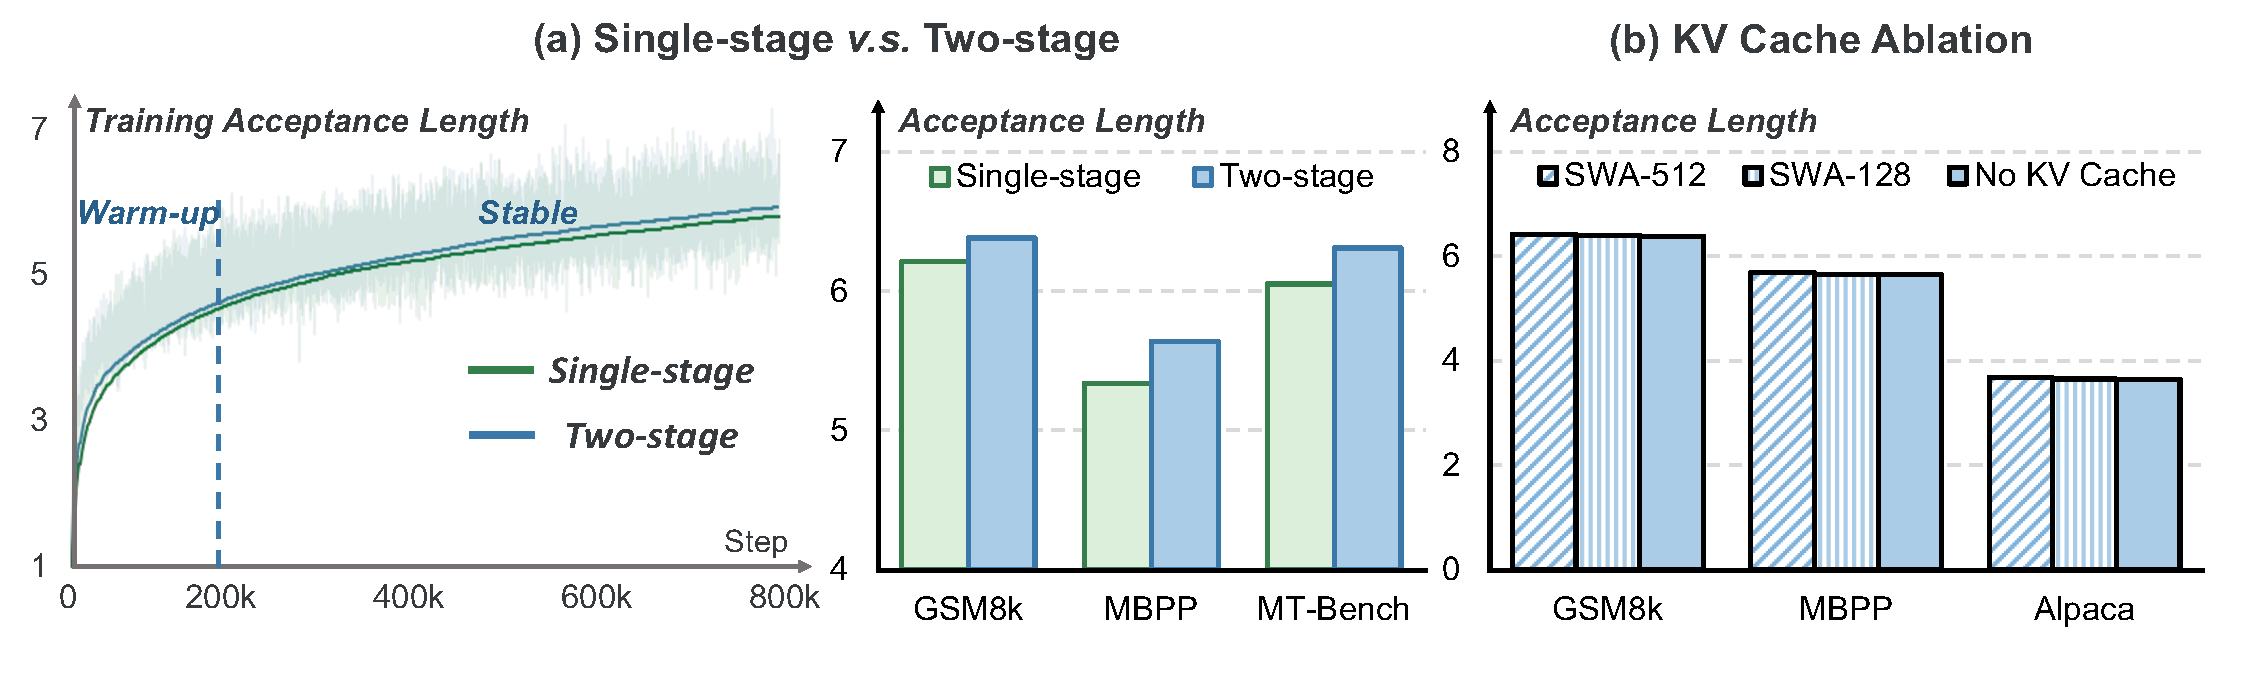
\includegraphics[width=\linewidth]{fig/ablation.pdf}
    \vspace{-20pt}
    \caption{Ablation on training strategy and KV cache.}
    \label{fig:ablation}
    % \vspace{-10pt}
\end{figure}

\textbf{Training strategy.}  Figure~\ref{fig:ablation}(a) compares our two-stage training strategy with direct single-stage training. The two-stage strategy consistently achieves higher acceptance length throughout the stable stage and improves the final performance. This result supports our motivation in Section~\ref{sec:DLite:train}: the history-aware isomorphic teacher provides an effective optimization bridge before direct alignment.

\textbf{Historical KV cache.} To examine whether historical draft states are necessary for accurate speculation, we additionally train two variants with sliding-window KV caches of 128 and 512 tokens using the same training data and setup as \we. As shown in Figure~\ref{fig:ablation}(b), after sufficient training, the three models achieve comparable acceptance lengths across the evaluated benchmarks. This suggests that historical KV states can facilitate prediction at earlier stages of training, but their advantage diminishes as the drafter learns to exploit contextual information transferred through the target hidden states. With sufficient training, \we can therefore achieve comparable quality without explicitly maintaining KV cache.



\textbf{Design space exploration.} We further explore several architectural design choices of \we, including the number of hidden states extracted from the target model, how multiple target hidden states are composed (feature-wise versus sequence-wise concatenation), and the rank of the lightweight sequential head. These dimensions jointly determine the trade-off between contextual representation capacity, drafting quality, and execution overhead. We use this design-space exploration in Appendix~\ref{app:dse} to determine the final configurations reported in Section~\ref{sec:exp:setup}.

\section{Conclusion}

In this work, we present \we, a history-free speculative decoding framework for agentic AI. \we removes the need for maintaining historical draft KV cache by directly reusing contextual hidden states from the target model and reformulating draft generation as local speculative prediction. On top of the history-free parallel backbone, a lightweight sequential head restores intra-block causal dependencies with low overhead, while a tailored two-stage training strategy addresses the optimization difficulty caused by the heterogeneous prediction structures of the draft and target models. Extensive experiments on general-purpose, long-context, and agentic workloads show that \we achieves \(2\sim6\) acceptance length and improves over the state-of-the-art semi-autoregressive drafter DSpark by up to \(70\%\), while eliminating historical draft KV-cache maintenance. These results demonstrate that removing redundant historical modeling from the drafter can simultaneously improve speculative decoding quality and system efficiency for emerging agentic workloads.

% \subsection*{AI use statement}

% (This section is \textbf{required} and does not count toward the page limit.)

% In this work, we used generative AI tools to 
% generate synthetic datasets,
% design or provide feedback on research methodology or experiments,
% assist with translation, 
% implement methods and interpret results.
% We have not used generative AI tools to 
% clean and reformat dataset. 
% And  
% help develop theoretical models or conceptual frameworks, 
% formulate mathematical claims, 
% provide critical ingredients for proving mathematical claims, 
% assist in the writing of proofs, 
% propose or refine hypotheses,  
% support qualitative and thematic data analysis 
% are not applicable to this work.
% Additionally, we used generative AI tools for create or modify scientific figures or images, suggest experimental parameters, create or edit software code, creation of artifacts, draft parts of a research paper, brainstorming, sourcing/searching for information, edit a research paper to improve readability, identify relevant literature, and suggest a structure for a research paper. We have reviewed all AI-assisted work. We take responsibility for the final content of this work,
% including text, claims or artifacts produced with the aid of generative AI.

% In this work, we used generative AI tools for generating synthetic training data, designing and providing feedback on research methodology and experiments, implementing methods, assisting with translation, and interpreting experimental results. We have not used generative AI tools for cleaning or reformatting datasets, and developing theoretical models or conceptual frameworks, formulating mathematical claims, providing critical ingredients for proving mathematical claims, assisting in the writing of proofs, proposing or refining hypotheses, and supporting qualitative or thematic data analysis are not applicable to this work. Additionally, we used generative AI tools for creating or modifying scientific figures, suggesting experimental parameters, creating or editing software code, creating research artifacts, drafting and editing parts of the manuscript, brainstorming, sourcing and searching for information, identifying relevant literature, improving readability, and suggesting the structure of the paper. We have reviewed all AI-assisted work. AI-assisted code and methodological suggestions were manually reviewed and validated by the authors, experimental interpretations were checked against the original results, and literature-related information was verified against the corresponding sources. We take responsibility for the final content of this work, including text, claims, or artifacts produced with the aid of generative AI.

% See the ICLR 2027 AI Policy for Authors for more details. This statement should
% not be more than 1 page.

% \subsection*{Ethics statement}

% (This section is \textbf{recommended} and does not count toward the page limit.)

% If authors feel that their paper submission raises questions regarding the Code
% of Ethics, they are encouraged to include a paragraph of Ethics Statement (at
% the end of the main text before references) to address potential concerns where
% appropriate. Topics include, but are not limited to, studies that involve human
% subjects, practices to data set releases, potentially harmful insights,
% methodologies and applications, potential conflicts of interest and sponsorship,
% discrimination/bias/fairness concerns, privacy and security issues, legal
% compliance, and research integrity issues (e.g., IRB, documentation, research
% ethics). This statement should not be more than 1 page.

% \subsection*{Reproducibility statement}

% (This section is \textbf{recommended} and does not count toward the page limit.)

% It is important that the work published in ICLR is reproducible. Authors are
% strongly encouraged to include a paragraph-long Reproducibility Statement at the
% end of the main text (before references) to discuss the efforts that have been
% made to ensure reproducibility. This paragraph should not itself describe
% details needed for reproducing the results, but rather reference the parts of
% the main paper, appendix, and supplemental materials that will help with
% reproducibility. For example, for novel models or algorithms, a link to an
% anonymous downloadable source code can be submitted as supplementary materials;
% for theoretical results, clear explanations of any assumptions and a complete
% proof of the claims can be included in the appendix; for any datasets used in
% the experiments, a complete description of the data processing steps can be
% provided in the supplementary materials. Each of the above are examples of
% things that can be referenced in the reproducibility statement.

% \subsubsection*{Author Contributions}
% If you'd like to, you may include  a section for author contributions as is done
% in many journals. This is optional and at the discretion of the authors.

\subsubsection*{Acknowledgments}
This work was sponsored by the National Natural Science Foundation of China (No. 62622406, 62674144, 62561160156) and Shanghai Rising-Star Program (No. 24QB2706200).

\bibliography{iclr2027_conference}
\bibliographystyle{iclr2027_conference}

\appendix
\section{Appendix}
\subsection{Training Details}

We train \we on the datasets described in Section~\ref{sec:exp:setup}. For all training data, we only use the original prompts and regenerate responses using the corresponding target model, ensuring that the supervision is consistent with the target distribution.

\textbf{Model configuration.} For Qwen3-4B and Qwen3-8B, the \we backbone contains 5 Transformer layers with hidden dimension \(2560/4096\). We extract 12/14 hidden states from the target model using sequence-wise composition. Specifically, we always retain the hidden states from the first and last layers, while uniformly sampling the remaining hidden states from the intermediate layers. The rank of lightweight sequential head is \(R=320/512\) for Qwen3-4B/8B, respectively. The speculative block length is set to \(K=7\).

\textbf{Training data.} Our training corpus contains approximately 1.9M samples in total, including 1.3M samples from Open-PerfectBlend and 600K samples from NVIDIA Nemotron Post-Training Dataset V2. We use only the prompts from these datasets and generate responses with the target model. The maximum sequence length is 4096, and each training sample contains 512 speculative blocks / anchors on average.

\textbf{Optimization.} We train \we using AdamW with a learning rate of $4 \times 10^{-4}$ and gradient clipping threshold 1.0. The global batch size is 32, with gradient accumulation of 1 step. We use cosine learning-rate decay with 0.04 warm-up ratio. Training is performed on 32 NVIDIA H800 GPUs.

\textbf{Two-stage training.} The positional weight decay $\gamma$ is set to 4. Training consists of a warm-up stage followed by a stable stage. In the warm-up stage, we first train the isomorphic history-aware teacher with the same data mentioned above using token-level cross-entropy for 8 epochs. We then train \we against this teacher using forward KL divergence for 2 epochs. In the stable stage, the history-aware teacher is removed and \we is directly optimized against the target model using
\[
\mathcal{L}_{\mathrm{stable}}
=
\lambda_{\mathrm{CE}}\mathcal{L}_{\mathrm{CE}}
+
\lambda_{\mathrm{TV}}\mathcal{L}_{\mathrm{TV}},
\]
where \(\lambda_{\mathrm{CE}}=0.1\) and \(\lambda_{\mathrm{TV}}=1\). The stable stage lasts for 6 epochs.



\subsection{Design Space exploration} \label{app:dse}
We conduct a design space exploration on Qwen3-8B to study three key architectural choices of \we: (1) the number of target hidden states used as contextual features, (2) the composition strategy for multiple target hidden states, and (3) the rank of the lightweight sequential head. To reduce the cost of design exploration, all variants in this section are trained on the same 80K-sample subset, while keeping the remaining training configurations unchanged. We evaluate the average acceptance length on Alpaca, GSM8K, MBPP, and Multi-Document QA, covering conversational, mathematical, coding, and long-context workloads.

\begin{table*}[h]
\centering
\caption{
Design space exploration of \we on Qwen3-8B.
All variants are trained on the same 80K-sample subset, and we report average acceptance length ($\tau$).
For the target hidden-state exploration, the first and last target layers are always included in addition to the sampled intermediate layers.
Unless otherwise specified, we use 14 target hidden states, sequence-wise hidden-state composition, and a sequential-head rank of 512.
Bold indicates the configuration adopted in the final model.
}
\label{tab:dse}
\resizebox{\textwidth}{!}{
\begin{tabular}{llccccc}
\toprule
\textbf{Dimension} &
\textbf{Configuration} &
\textbf{Alpaca} &
\textbf{GSM8K} &
\textbf{MBPP} &
\textbf{Multi-Doc QA} &
\textbf{Avg. $\tau$} \\
\midrule

\multirow{5}{*}{\textbf{Target Hidden States}}
& 7
& 2.34 & 4.36 & 3.63 & 2.22 & 3.14 \\

& 9
& 2.42 & 4.40 & 3.75 & 2.24 & 3.20 \\

& \textbf{14}
& \textbf{2.63} & \textbf{4.53} & \textbf{3.76} & \textbf{2.28} & \textbf{3.30} \\

& 20
& 2.62 & 4.55 & 3.74 & 2.26 & 3.29 \\

& 36
& 2.58 & 4.51 & 3.71 & 2.26 & 3.27 \\

\midrule

\multirow{2}{*}{\textbf{Hidden Composition}}
& Feature-wise
& 2.20 & 4.28 & 3.50 & 2.16 & 3.04 \\

& \textbf{Sequence-wise}
& \textbf{2.63} & \textbf{4.53} & \textbf{3.76} & \textbf{2.28} & \textbf{3.30} \\

\midrule

\multirow{5}{*}{\textbf{Sequential-Head Rank}}
& 256 ($1/16D$)
& 2.48 & 4.40 & 3.61 & 2.16 & 3.16 \\

& \textbf{512 ($1/8D$)}
& \textbf{2.63} & \textbf{4.53} & \textbf{3.76} & \textbf{2.28} & \textbf{3.30} \\

& 1024 ($1/4D$)
& 2.64 & 4.55 & 3.80 & 2.28 & 3.32 \\

& 2048 ($1/2D$)
& 2.64 & 4.53 & 3.82 & 2.28 & 3.32 \\

& 4096 ($D$)
& 2.64 & 4.56 & 3.82 & 2.30 & 3.33 \\

\bottomrule
\end{tabular}
}
\end{table*}


\textbf{Number of target hidden states.} Table~\ref{tab:dse} shows that increasing the number of target hidden states initially leads to clear improvements in acceptance length. The gains, however, quickly saturate: increasing the number from 7 to 14 improves performance consistently across all four workloads, while using 20 or 36 hidden states provides little or no additional benefit. This suggests that a moderate number of intermediate target representations is sufficient to capture complementary contextual information, while further increasing the number of features introduces redundant representations and additional computation.

\textbf{Hidden-state composition.} We further compare two ways of combining hidden states extracted from different target layers. Sequence-wise concatenation treats representations from different layers as separate input elements, while feature-wise concatenation concatenates them along the hidden dimension. Sequence-wise concatenation consistently outperforms feature-wise concatenation across all evaluated workloads, increasing the average acceptance length from 3.04 to 3.30. We therefore adopt sequence-wise composition in \we. This result also supports the use of depth embeddings in Section~\ref{sec:DLite:arch}, which explicitly identify the source layers of hidden states when they are presented as separate inputs.

\textbf{Sequential-head rank.} Finally, we vary the rank of the lightweight sequential head from 1/16 of the hidden dimension (256) to the full hidden dimension (4096). Increasing the rank from 256 to 512 yields a noticeable improvement in drafting quality while increasing the end-to-end latency by only 0.3\%, whereas larger ranks provide only marginal gains while introducing substantial computational overhead. This suggests that the information required by the draft model can be sufficiently resolved in a low-rank space. For example, the average acceptance length increases from 3.16 at rank 256 to 3.30 at rank 512, but only reaches 3.33 with the full 4096-dimensional head. Considering the additional sequential computation introduced by a larger rank and the diminishing performance gains, we choose a relatively small rank to balance drafting quality and execution efficiency.

\paragraph{Implementation details.}
We evaluate \we on four agent-oriented benchmarks using Qwen3-4B and Qwen3-8B targets. For SWE-Bench, we use 50 prompts from 64K settings (40K--64K input tokens). For AgentLongBench, we use 50 prompts from the 64K setting (55.5K--74.1K input tokens). For MemoryAgentBench, we select 100 FactConsolidation, 50 EventQA, and 30 free-form DetectiveQA questions (66K--118K input tokens), constructing one independent long-context prompt per question. For BFCL, we use 41 sessions from the \texttt{multi\_turn\_long\_context} category, run its multi-turn tool-execution harness through a local OpenAI-compatible inference adapter, and aggregate model calls whose input exceeds 32K tokens. BFCL tool-execution time is excluded. 


\end{document}
